\documentclass[onecolumn]{article}
\usepackage[T1]{fontenc} % make copy/paste of ^ in verbatim work properly in code
\usepackage{lmodern}     % make copy/paste of ^ in verbatim work properly in code
\usepackage{graphicx,color,psfrag}
\usepackage[caption=false,font=footnotesize]{subfig}
\usepackage{amsmath,amssymb}
\usepackage{cite}
\usepackage{verbatim}
\usepackage{listings}
\usepackage{upquote}   % Make copy/paste of single quotes in verbatim work properly in code, use \char"0D inside text
\usepackage{paralist}  % single-spaced lists via compactitem
\usepackage{enumitem}  % single-spaced enumerations via manual control

\usepackage{longtable} % multi-page tables
\usepackage[title,titletoc,toc]{appendix}

\usepackage[multidot]{grffile} % allow dots in graphics filenames
\usepackage[usenames,dvipsnames]{xcolor}
\definecolor{DarkGreen}{rgb}{0,0.35,0.1} % because the default light green is pretty hard to read, don't you think?
\usepackage[pagebackref=true, breaklinks=true, colorlinks=true, bookmarks=true, citecolor=DarkGreen, linkcolor=DarkGreen, urlcolor=DarkGreen]{hyperref}
\usepackage{url}
\usepackage{breakurl}
\usepackage{fancyvrb}

%---Repeating a variable number of times---
\makeatletter
\newcommand{\Repeat}[1]{%
    \expandafter\@Repeat\expandafter{\the\numexpr #1\relax}%
}
\def\@Repeat#1{%
    \ifnum#1>0
        \expandafter\@@Repeat\expandafter{\the\numexpr #1-1\expandafter\relax\expandafter}%
    \else
        \expandafter\@gobble
    \fi
}
\def\@@Repeat#1#2{%
    \@Repeat{#1}{#2}#2%
}
\makeatother
%------------------------------------------

\title{
Light Field Toolbox for Matlab\\
{\large Version 0.5.0}
}


\author{Copyright (c) 2013-2020 Donald G. Dansereau}
\date{}
\usepackage{bm}  % bolding with \bm

\DeclareMathSymbol{\Gamma}{\mathalpha}{letters}{"00}
\DeclareMathSymbol{\Delta}{\mathalpha}{letters}{"01}
\DeclareMathSymbol{\Theta}{\mathalpha}{letters}{"02}
\DeclareMathSymbol{\Lambda}{\mathalpha}{letters}{"03}
\DeclareMathSymbol{\Xi}{\mathalpha}{letters}{"04}
\DeclareMathSymbol{\Pi}{\mathalpha}{letters}{"05}
\DeclareMathSymbol{\Sigma}{\mathalpha}{letters}{"06}
\DeclareMathSymbol{\Upsilon}{\mathalpha}{letters}{"07}
\DeclareMathSymbol{\Phi}{\mathalpha}{letters}{"08}
\DeclareMathSymbol{\Psi}{\mathalpha}{letters}{"09}
\DeclareMathSymbol{\Omega}{\mathalpha}{letters}{"0A}

\DeclareMathOperator{\tr}{Tr}
\DeclareMathOperator{\MSE}{MSE}
\DeclareMathOperator{\E}{E}

\newcommand{\rpm}{\raisebox{.2ex}{$\scriptstyle\pm$}}  % better plus or minus

%\newcommand{\vect}[1]{\vec{#1}}  % arrow on top
\newcommand{\vect}[1]{\bm{#1}}
\newcommand{\const}[1]{\mathrm{#1}}
\newcommand{\constvect}[1]{\bm{\mathrm{#1}}}
\newcommand{\mat}[1]{\bm{\mathalpha{#1}}}   % bold matrices
\newcommand{\constmat}[1]{\bm{\mathrm{#1}}} % bold matrices
%\newcommand{\mat}[1]{{\mathalpha{#1}}}     % not bold matrices
%\newcommand{\constmat}[1]{{\mathrm{#1}}}   % not bold matrices
\newcommand{\abs}[1]{\left|#1\right|}
\newcommand{\norm}[1]{\left\|#1\right\|}
\newcommand{\unitvect}[1]{\vect{\hat{#1}}}
\newcommand{\sgn}{\operatorname{sgn}}
%\newcommand\trans[1]{#1^{\mathsf{\intercal}}}
%\newcommand\trans[1]{#1^{\mathsf{T}}}
%\newcommand\trans[1]{#1^{\top}}
\newcommand\trans[1]{#1^{\scriptscriptstyle\mathsf{T}}}
%\newcommand\negative[1]{\,{\text{-}#1}}
%\newcommand\negative[1]{\mathord{-}{#1}}
\newcommand\negative[1]{{\text{-}#1}}
\newcommand\negtrans[1]{#1^{\negative{\scriptscriptstyle\mathsf{T}}}}
\newcommand\sub[1]{_{\scriptscriptstyle\mathit{#1}}}
\newcommand\subup[1]{_{\scriptscriptstyle\mathrm{#1}}}
\newcommand\super[1]{^{\scriptscriptstyle\mathit{#1}}}
\newcommand\superup[1]{^{\scriptscriptstyle\mathrm{#1}}}
\newcommand{\argmin}{\operatornamewithlimits{argmin}}

% upright lowercase greek characters, from http://www-zeus.desy.de/~wing/dstar_dis_final_paper/submit_hep_ex/LaTeX/styles/upgreek.sty
% alternatives: http://www.superstrate.net/useful/useful.html, or the built-in upgreek.sty, but it doesn't look as nice
%-----------------------------------------------------------------------
%  define symbol fonts 
%-----------------------------------------------------------------------
\DeclareSymbolFont{EUr}{U}{eur}{m}{n}
\DeclareSymbolFont{EUb}{U}{eur}{b}{n}
%-----------------------------------------------------------------------
%  define upright greek letters
%-----------------------------------------------------------------------
\DeclareMathSymbol{\upGamma}{\mathord}{EUr}{"00}
\DeclareMathSymbol{\upDelta}{\mathord}{EUr}{"01}
\DeclareMathSymbol{\upTheta}{\mathord}{EUr}{"02}
\DeclareMathSymbol{\upLambda}{\mathord}{EUr}{"03}
\DeclareMathSymbol{\upXi}{\mathord}{EUr}{"04}
\DeclareMathSymbol{\upPi}{\mathord}{EUr}{"05}
\DeclareMathSymbol{\upSigma}{\mathord}{EUr}{"06}
\DeclareMathSymbol{\upUpsilon}{\mathord}{EUr}{"07}
\DeclareMathSymbol{\upPhi}{\mathord}{EUr}{"08}
\DeclareMathSymbol{\upPsi}{\mathord}{EUr}{"09}
\DeclareMathSymbol{\upOmega}{\mathord}{EUr}{"0A}
\DeclareMathSymbol{\upalpha}{\mathord}{EUr}{"0B}
\DeclareMathSymbol{\upbeta}{\mathord}{EUr}{"0C}
\DeclareMathSymbol{\upgamma}{\mathord}{EUr}{"0D}
\DeclareMathSymbol{\updelta}{\mathord}{EUr}{"0E}
\DeclareMathSymbol{\upepsilon}{\mathord}{EUr}{"0F}
\DeclareMathSymbol{\upzeta}{\mathord}{EUr}{"10}
\DeclareMathSymbol{\upeta}{\mathord}{EUr}{"11}
\DeclareMathSymbol{\uptheta}{\mathord}{EUr}{"12}
\DeclareMathSymbol{\upiota}{\mathord}{EUr}{"13}
\DeclareMathSymbol{\upkappa}{\mathord}{EUr}{"14}
\DeclareMathSymbol{\uplambda}{\mathord}{EUr}{"15}
\DeclareMathSymbol{\upmu}{\mathord}{EUr}{"16}
\DeclareMathSymbol{\upnu}{\mathord}{EUr}{"17}
\DeclareMathSymbol{\upxi}{\mathord}{EUr}{"18}
\DeclareMathSymbol{\uppi}{\mathord}{EUr}{"19}
\DeclareMathSymbol{\uprho}{\mathord}{EUr}{"1A}
\DeclareMathSymbol{\upsigma}{\mathord}{EUr}{"1B}
\DeclareMathSymbol{\uptau}{\mathord}{EUr}{"1C}
\DeclareMathSymbol{\upupsilon}{\mathord}{EUr}{"1D}
\DeclareMathSymbol{\upphi}{\mathord}{EUr}{"1E}
\DeclareMathSymbol{\upchi}{\mathord}{EUr}{"1F}
\DeclareMathSymbol{\uppsi}{\mathord}{EUr}{"20}
\DeclareMathSymbol{\upomega}{\mathord}{EUr}{"21}
\DeclareMathSymbol{\upvarepsilon}{\mathord}{EUr}{"22}
\DeclareMathSymbol{\upvartheta}{\mathord}{EUr}{"23}
\DeclareMathSymbol{\upvaromega}{\mathord}{EUr}{"24}
\DeclareMathSymbol{\upvarphi}{\mathord}{EUr}{"27}

%-----------------------------------------------------------------------
%  define bold upright greek letters
%-----------------------------------------------------------------------
\DeclareMathSymbol{\UpGamma}{\mathord}{EUb}{"00}
\DeclareMathSymbol{\UpDelta}{\mathord}{EUb}{"01}
\DeclareMathSymbol{\UpTheta}{\mathord}{EUb}{"02}
\DeclareMathSymbol{\UpLambda}{\mathord}{EUb}{"03}
\DeclareMathSymbol{\UpXi}{\mathord}{EUb}{"04}
\DeclareMathSymbol{\UpPi}{\mathord}{EUb}{"05}
\DeclareMathSymbol{\UpSigma}{\mathord}{EUb}{"06}
\DeclareMathSymbol{\UpUpsilon}{\mathord}{EUb}{"07}
\DeclareMathSymbol{\UpPhi}{\mathord}{EUb}{"08}
\DeclareMathSymbol{\UpPsi}{\mathord}{EUb}{"09}
\DeclareMathSymbol{\UpOmega}{\mathord}{EUb}{"0A}
\DeclareMathSymbol{\Upalpha}{\mathord}{EUb}{"0B}
\DeclareMathSymbol{\Upbeta}{\mathord}{EUb}{"0C}
\DeclareMathSymbol{\Upgamma}{\mathord}{EUb}{"0D}
\DeclareMathSymbol{\Updelta}{\mathord}{EUb}{"0E}
\DeclareMathSymbol{\Upepsilon}{\mathord}{EUb}{"0F}
\DeclareMathSymbol{\Upzeta}{\mathord}{EUb}{"10}
\DeclareMathSymbol{\Upeta}{\mathord}{EUb}{"11}
\DeclareMathSymbol{\Uptheta}{\mathord}{EUb}{"12}
\DeclareMathSymbol{\Upiota}{\mathord}{EUb}{"13}
\DeclareMathSymbol{\Upkappa}{\mathord}{EUb}{"14}
\DeclareMathSymbol{\Uplambda}{\mathord}{EUb}{"15}
\DeclareMathSymbol{\Upmu}{\mathord}{EUb}{"16}
\DeclareMathSymbol{\Upnu}{\mathord}{EUb}{"17}
\DeclareMathSymbol{\Upxi}{\mathord}{EUb}{"18}
\DeclareMathSymbol{\Uppi}{\mathord}{EUb}{"19}
\DeclareMathSymbol{\Uprho}{\mathord}{EUb}{"1A}
\DeclareMathSymbol{\Upsigma}{\mathord}{EUb}{"1B}
\DeclareMathSymbol{\Uptau}{\mathord}{EUb}{"1C}
\DeclareMathSymbol{\Upupsilon}{\mathord}{EUb}{"1D}
\DeclareMathSymbol{\Upphi}{\mathord}{EUb}{"1E}
\DeclareMathSymbol{\Upchi}{\mathord}{EUb}{"1F}
\DeclareMathSymbol{\Uppsi}{\mathord}{EUb}{"20}
\DeclareMathSymbol{\Upomega}{\mathord}{EUb}{"21}
\DeclareMathSymbol{\Upvarepsilon}{\mathord}{EUb}{"22}
\DeclareMathSymbol{\Upvartheta}{\mathord}{EUb}{"23}
\DeclareMathSymbol{\Upvaromega}{\mathord}{EUb}{"24}
\DeclareMathSymbol{\Upvarphi}{\mathord}{EUb}{"27}

%% New definition of square root:
%% it renames \sqrt as \oldsqrt
%\let\oldsqrt\sqrt
%% it defines the new \sqrt in terms of the old one
%\def\sqrt{\mathpalette\DHLhksqrt}
%\def\DHLhksqrt#1#2{%
%\setbox0=\hbox{$#1\oldsqrt{#2\,}$}\dimen0=\ht0
%\advance\dimen0-0.2\ht0
%\setbox2=\hbox{\vrule height\ht0 depth -\dimen0}%
%{\box0\lower0.4pt\box2}}

%% comma separation for large numbers, e.g. 1,000,000 
\newcount\ppnum
\newcommand\ppnumber[1]{%
        \ppnum=#1\relax
        \ifnum\ppnum<0
                $-$%
                \ppnum=-\ppnum
        \fi
        \let\pptemp\empty
        \loop\ifnum\ppnum>999
                \count255=\ppnum
                \divide\ppnum by1000
                \count255=\numexpr \count255 - 1000*\ppnum \relax
                \edef\pptemp{,\!\ifnum\count255<100 0\ifnum\count255<10 0\fi\fi
                             \the\count255 \pptemp}%
        \repeat
        \the\ppnum
        \pptemp
}
 % for iso-standard math

% stop breaking inline equations across lines
%\relpenalty=9999  
%\binoppenalty=9999
%% window/orphan control
\widowpenalty=10000
\clubpenalty=10000

% Shortcuts for building the function reference
\newcommand{\NewTag}{\protect{~\color{red} \tiny NEW}}
\newcommand{\NewText}{\protect{~\color{red} \footnotesize NEW}}
\newcommand{\DeclareFunction}[1]{\hypertarget{#1}{#1}}
\newcommand{\CiteFunc}[1]{\hyperlink{#1}{\small #1}}
\newcommand{\SupFunction}[1]{{\small #1}}

\newcommand{\NewFunctionHeading}[1]{
\hspace{-1.5em}\begin{minipage}[t]{\linewidth}
\noindent\rule{\linewidth}{\arrayrulewidth}
\vspace{0.5em}\hspace{1pt}\textbf{\large #1}\\[-1.1em]
\rule{\linewidth}{\arrayrulewidth}\par\vspace{0.2em}
}

\newcommand{\NewFunctionEntry}[3]{%
\vspace{0.4em}%
	\hspace{1em}\begin{minipage}[t]{\linewidth}%
	\textbf{\DeclareFunction{#1}#2}%
	\end{minipage}\vspace{0.2em}\par
	\hspace*{3em}\begin{minipage}[t]{0.9\linewidth}%
	\protect #3 \vspace{0.4em}
	\end{minipage}%
	\par%
}

\newcommand{\EndFunctionHeading}{
\end{minipage}\vspace{1em}\par
}

% Shortcuts for creating an annotated folder structure
\newcommand{\NewAnnotatedTree}[1]{\vspace{1em}\noindent\begin{tabular}{*{#1}{p{0.1em}}cp{6.5cm}}}
\newcommand{\EndAnnotatedTree}{\end{tabular}\vspace{1em}}
\newcommand{\AnnotatedTreeEntry}[4]{\Repeat{#1}{&}\multicolumn{#2}{l}{\SymbolText{#3}} & \small #4}

\newcommand{\SymbolText}[1]{\texttt{\small #1}}

\RecustomVerbatimEnvironment
{Verbatim}{Verbatim}
{formatcom={\footnotesize}, fontfamily=courier}

\begin{document}

\maketitle
\thispagestyle{empty}\pagestyle{plain}

%-----------------------------
This is a toolbox for working with light field imagery in MATLAB. Features include loading, visualizing, and filtering light fields, and decoding, calibration, and rectification of lenslet-based imagery.

The most recent release and development versions are here: \url{https://github.com/doda42/LFToolbox}. 

The complementary LiFF light field feature toolbox is here: \url{http://dgd.vision/Tools/LiFF}.

%-----------------------------
\vspace{1em}\noindent\textbf{\large{What's New  / Development Plan}}\vspace{0.5em}

For a complete list, see CHANGELOG.txt. v0.5 highlights:
\begin{itemize}[leftmargin=2.8em,itemsep=0em,rightmargin=0.5cm]
\item Linear refocus super-resolution using \CiteFunc{LFFiltShiftSum}, see \CiteFunc{LFDemoRefocusSuperres}
\item New display functions \CiteFunc{LFDispLawnmower}, \CiteFunc{LFDispTiles}, \CiteFunc{LFDispTilesSubfigs}, \CiteFunc{LFDispProj}, \CiteFunc{LFDispProjSubfigs}
\item \CiteFunc{LFReadESLF}, \CiteFunc{LFWriteESLF}
\item Improved decode performance and speed
\item Improved calibration accuracy
\item LFDisp* functions are better behaved, now display in the active figure window
\end{itemize}


Future plans include more significant changes to lenslet-based decode and calibration, and support for a broader range of cameras.

%-----------------------------
\vspace{1em}\noindent\textbf{\large{Compatibility}}\vspace{0.5em}

\textbf{Reverse-compatibility}: Changes to interfaces have been minimised, \CiteFunc{LFDispVidCirc} is the main exception, with a new parameter structure.

Previously generated calibration files should be re-generated, and to benefit from performance improvements to decoding, white images should be re-generated.  See Appendix~\ref{sect_Upgrading} for details.

\textbf{Matlab}: LFToolbox 0.5 was written in MATLAB 2020a, but should be compatible with earlier versions.

\textbf{File Formats}: The toolbox can load gantry / array-style folders of images, ESLF files, and raw lenslet-based images.

\textbf{Plenoptic 1.0} cameras are supported through decoding, calibration, and rectification of imagery. Functions are most easily applied to Lytro imagery. The toolbox can also be applied to other lenslet-based Plenoptic 1.0 cameras, but this is not yet well documented. Calibration of Lytro Illum cameras is experimental.

\textbf{Plenoptic 2.0} cameras are not well supported. Use with some cameras is possible but not well documented. Multi-focal lenslet-based cameras are not well supported.

\textbf{Lytro Software}: The toolbox is compatible with files generated using Lytro Desktop 4 and 3.

%-----------------------------
\vspace{1em}\noindent\textbf{\large{Contributing / Feedback}}\vspace{0.5em}

Suggestions, bug reports, code improvements and new functionality are welcome -- email \SymbolText{Donald.Dansereau+LFToolbox} \small{at} \SymbolText{gmail} \small{dot} \SymbolText{com}.

%-----------------------------
\vspace{1em}\noindent\textbf{\large{Acknowledgments}}\vspace{0.5em}

Parts of the code were taken with permission from the Camera Calibration Toolbox for Matlab by Jean-Yves Bouguet, with contributions from Pietro Perona and others; and from the JSONlab Toolbox by Qianqian Fang and others. LFFigure was originally by Daniel Eaton. The LFP reader is based in part on Nirav Patel and Doug Kelley's LFP readers. Thanks to Michael Tao for help and samples for decoding Illum imagery.

%-----------------------------
\vspace{1em}\noindent\textbf{\large{Citing}}\vspace{0.5em}

The appropriate citations for decoding, calibration and rectification and the volumetric focus (hyperfan) filter are (see the README file for bibtex): \vspace{0.5em} \\ 
\footnotesize [1] \small{D.\ G.\ Dansereau, O.\ Pizarro, and S.\ B.\ Williams, ``Decoding, calibration and rectification for lenselet-based plenoptic cameras,'' in Computer Vision and Pattern Recognition (CVPR), IEEE Conference on. IEEE, Jun 2013.} \vspace{0.5em} \\ 
\footnotesize [2] \small{D.\ G.\ Dansereau, O.\ Pizarro, and S.\ B.\ Williams, ``Linear Volumetric Focus for Light Field Cameras,'' in ACM Transactions on Graphics (TOG), vol. 34, no. 2, 2015.}

\newpage
\tableofcontents
\newpage

%-----------------------------
\section{Installation}
\label{sect_Installation}

\subsection{Installing the Toolbox}

Prior to installation, remove / uninstall any previous light field toolbox versions. There are three main options for installation:
\begin{enumerate}[leftmargin=2.2em,itemsep=0em,rightmargin=0.5cm]
\item Install as a ``toolbox'' via the Mathworks site; this handles path setup automatically
\item Download a .zip file from either the Mathworks site or Github
\item Clone the git repo and checkout the release or a development branch
\end{enumerate}

For options 2 and 3, put the toolbox files in an appropriate location, and run the convenience function \CiteFunc{LFMatlabPathSetup} to set up the Matlab path. This must be re-run every time Matlab restarts, so consider adding a line to \SymbolText{startup.m}, e.g.\ \begin{Verbatim}
run('~/MyMatlabCode/LFToolbox0.5/LFMatlabPathSetup.m')
\end{Verbatim}

To check your installation:

\begin{itemize}[leftmargin=2.8em,itemsep=0em,rightmargin=0.5cm]
\item Run \SymbolText{LFToolboxVersion} to check the toolbox version
\item Type \SymbolText{which LFToolboxVersion} to confirm the path to the toolbox folder
\item Type \SymbolText{help <toolbox folder name>}, e.g. \SymbolText{help LFToolbox0.5} to display a list of toolbox functions
\end{itemize} 

\subsection{Downloading Samples}

\begin{itemize}[leftmargin=2.2em,itemsep=0em,rightmargin=0.5cm]
\item LFToolbox v0.5 Sample Pack, including example ESLF and Lytro F01 and Illum images: \url{http://www-personal.acfr.usyd.edu.au/donald/LFToolbox0.5_Samples.zip}
\item Small Sample Calibration: \url{http://www-personal.acfr.usyd.edu.au/ddan1654/PlenCalSmallExample.zip}
\item Gantry-style and large collections of ESLF files at Stanford: \url{http://lightfields.stanford.edu}
\end{itemize}

\subsection{Additional Resources}

\begin{itemize}
\item Questions about the toolbox should go to the Light Field Vision mailing list: \url{https://groups.google.com/forum/#!forum/lightfieldvision}
\item Additional datasets and community links: \url{http://dgd.vision/Tools/LFToolbox}
\end{itemize}

%-----------------------------
\section{Conventions}
\label{sect_Conventions}

\subsection{Optional Function Arguments}

Many toolbox functions accept optional function arguments, taking on default values if no value is provided. Simply omit arguments at the end of the list, or pass an empty array \SymbolText{[]} within the list. For example, for the function

\begin{Verbatim}
LFDispMousePan( LF, ScaleFactor, InitialViewIdx, Verbose )
\end{Verbatim}
all arguments except the first are optional. Any of the following are valid:
\begin{Verbatim}
LFDispMousePan( LF ) 
LFDispMousePan( LF, 4 )               % set a scale factor of 4
LFDispMousePan( LF, 4, [3,3] )        % .. also set initial view index 3,3
LFDispMousePan( LF, [], [3,3] )       % initial view 3,3, default scale
LFDispMousePan( LF, [], [3,3], true ) % initial view 3,3, verbose on
LFDispMousePan( LF, 4, [], true )     % scale factor 4, verbose on
\end{Verbatim}

\subsection{Struct Arguments}

Some functions accept structs of arguments. A helpful shorthand for calling these is using MATLAB's \SymbolText{struct} function, that allows inline struct construction, e.g.
\begin{Verbatim}
LFUtilDecodeLytroFolder('Images', [], struct('OptionalTasks', 'ColourCorrect'))
\end{Verbatim}

See the help for \CiteFunc{LFUtilDecodeLytroFolder} for more examples of these argument-passing conventions.

\subsubsection{Continuous vs Discrete Indices}
In formal presentation, discrete indices $i,j,k,l$ are distinct from continuous spatial coordinates $s,t,u,v$. In the toolbox, when it is clear that the light field is sampled, the latter is generally understood to refer to sample indices.

\subsection{Light Field Indexing}

In MATLAB, to index a 2D colour image $I$ at the coordinates $x, y, c$ corresponding to horizontal position, vertical position, and colour, we use the indexing order $I( y,x, c )$. 

Generalizing this to a 4D light field $L$ which we wish to index at the horizontal, vertical ray position $s,t$, horizontal, vertical ray direction $u,v$, and colour channel $c$, we use the indexing order $L( t,s, v,u, c)$.

\subsubsection{Colour Channels}

Colour light fields have at least three colour channels, one for each of red, green, and blue. The toolbox can also handle monochrome light fields, with a single colour channel. 

For light fields that also have per-pixel weight information, there is an additional colour channel. Weight indicates confidence, so for example a pixel that is significantly amplified to compensate for vignetting will have a proportionally lower weight because we are less confident of its true value. A weight of zero means we do not know the value of the pixel.

\subsection{Two-Plane Parameterization}

The intrinsic matrices generated through calibration use a \emph{relative} two-plane parameterization, with a plane separation $D = 1 \const{m}$. This maps each pixel index $[i,j,k,l]$ to a corresponding ray in space $[s,t,u,v]$, where each of $s,t,u$ and $v$ is measured in meters. This combination unambiguously defines each ray in metric space including scale.


%-----------------------------
\section{A Quick Tour}
\label{sect_QuickTour}
%-----------------------------
\subsection{Working with Lytro Light Fields}
\label{sect_DecodingLytro}

\subsubsection{Decoding? Calibration? Rectification?}

The toolbox uses the following terminology:
\begin{enumerate}[leftmargin=1.5em,rightmargin=0.5cm]
\item \textbf{Decoding}: The lenslet array encodes the 4D light field onto a 2D sensor, and decoding undoes this process.
\item \textbf{Calibration}: This is characterizing the camera's optics to map each measured pixel to a ray in space.
\item \textbf{Rectification}: Removing distortions in the decoded light field to simplify the pixel-to-ray mapping to a linear relationship. In the simplest case, the resulting light field looks like what an array of parallel pinhole cameras would measure.
\end{enumerate}
See Sect.~\ref{sect_DecodingInDetail} and [1] for further details.

\subsubsection{Decoding the Samples}
\begin{enumerate}[leftmargin=1.5em,rightmargin=0.5cm]

\item \textbf{Install} the LF Toolbox and following the instructions in Sect.~\ref{sect_Installation}.

\item \textbf{Download} the sample light field pack at \url{http://www-personal.acfr.usyd.edu.au/ddan1654/LFToolbox0.5_Samples.zip} and decompress into its own folder. The samples folder structure was chosen for easy addition of your own cameras and calibrations:

\NewAnnotatedTree{6}
\AnnotatedTreeEntry{0}{7}{Samples}{Top level of samples}\\
\AnnotatedTreeEntry{1}{6}{Images}{Sample light field images}\\
\AnnotatedTreeEntry{2}{5}{ESLF}{ESLF images}\\
\AnnotatedTreeEntry{2}{5}{F01}{F01 images}\\
\AnnotatedTreeEntry{2}{5}{Illum}{Illum images}\\
\AnnotatedTreeEntry{1}{6}{Cameras}{Stores info for one or more cameras}\\
\AnnotatedTreeEntry{2}{5}{A000424242}{Camera used to measure F01 samples}\\
\AnnotatedTreeEntry{3}{4}{CalZoomedOutFixedFoc}{A single calibration result}\\
\AnnotatedTreeEntry{3}{4}{WhiteImages}{White images for the F01 camera}\\
\AnnotatedTreeEntry{2}{5}{B5143300780}{Camera used to measure Illum samples}\\
\AnnotatedTreeEntry{3}{4}{WhiteImages}{White images for the Illum camera}\\
\EndAnnotatedTree

\item \textbf{\SymbolText{cd <sample folder>}} inside MATLAB to change to the top level of the samples folder.  If you are in the correct location, the Matlab command \SymbolText{ls} should list the top-level folders and README file:
\begin{Verbatim}
Images   Cameras   README
\end{Verbatim}

\begin{figure}[tbh]
	\centering
	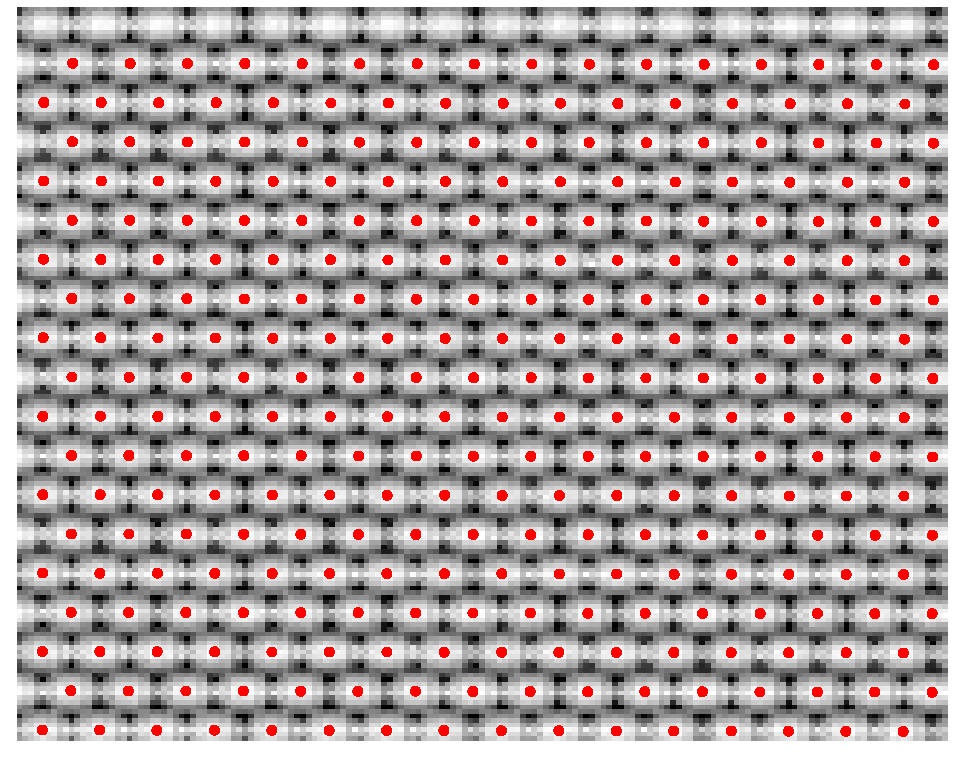
\includegraphics[width=0.5\textwidth]{Figs/ExampleWhiteImageLabeled}
	\caption{Example of a white (flat-field) image showing estimated lenslet centers as red dots.}
	\label{fig_WhiteImage}
\end{figure}

\item \textbf{Run \CiteFunc{LFUtilProcessWhiteImages}} to build a white image database. This searches the \SymbolText{Cameras} folder for white (flat-field) images, generating a lenslet grid model for each -- the grid models are saved as \SymbolText{*.grid.json}. The database of white images is saved as \SymbolText{Cameras/WhiteFileDatabase.mat}, and is used in selecting the appropriate white image for decoding each light field. 

Samples ship with precomputed \SymbolText{.grid.json} files. These files may be removed in order to force their re-generation.  When doing so, for each lenslet grid model a set of figures similar to Fig.~\ref{fig_WhiteImage} will be presented for visual confirmation that the grid model is a good fit. Each figure shows a small subset of the whole frame to allow close inspection of the lenslets. Five such images are shown, one for each image corner and one for the central portion of the image. Each red dot should appear near the center of a lenslet, as depicted in Fig.~\ref{fig_WhiteImage}.

\item \textbf{Run \CiteFunc{LFUtilDecodeLytroFolder}} to decode the sample light fields. The script searches the \SymbolText{Images} folder and its sub-folders for light fields and decodes each.  By default it searches for all compatible Lytro light field formats, including \SymbolText{lfp} and \SymbolText{raw}.

The decoding process selects the appropriate white image for each light field and saves the decoded 4D light fields, \SymbolText{*\_\_Decoded.mat}, and thumbnail, \SymbolText{*.png}, alongside the input images. A thumbnail of each light field is also displayed as it is decoded. Thumbnails are histogram-adjusted, but the saved light field is not. Example thumbnails are shown in Fig.~\ref{fig_ExampleDecodeAndColourCorrectOutput}.

\begin{figure}[tbh]
	\centering
	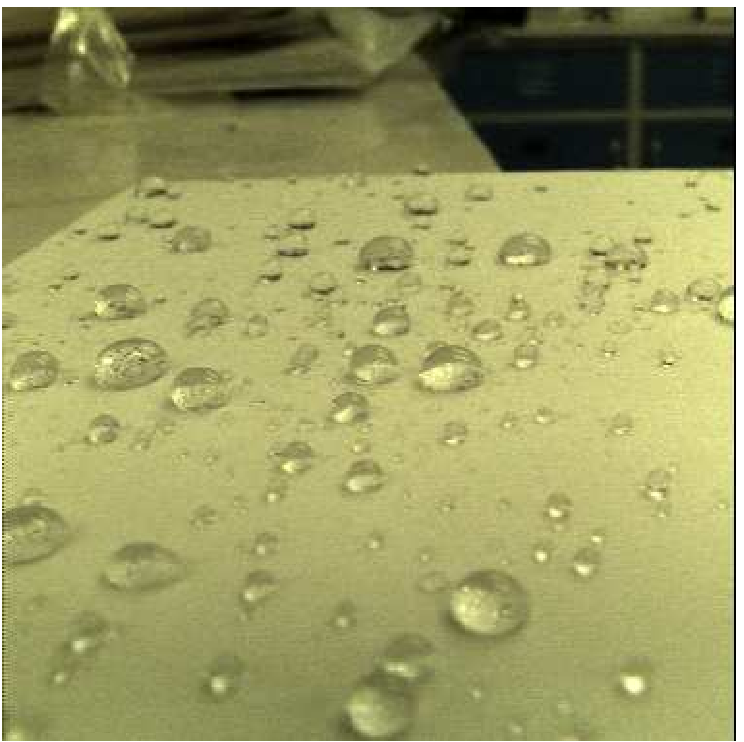
\includegraphics[width=0.32\textwidth]{Figs/Sample1}
	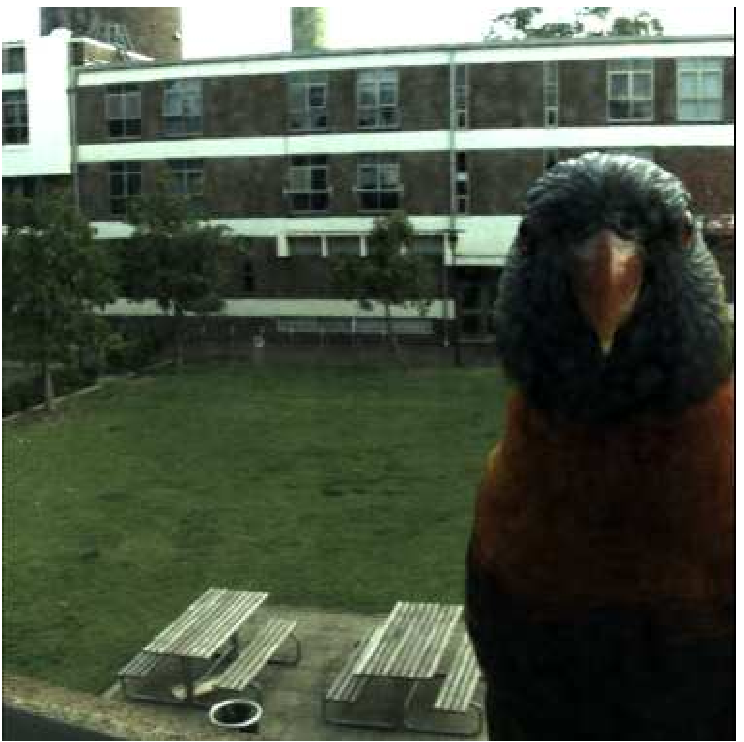
\includegraphics[width=0.32\textwidth]{Figs/Sample2}
	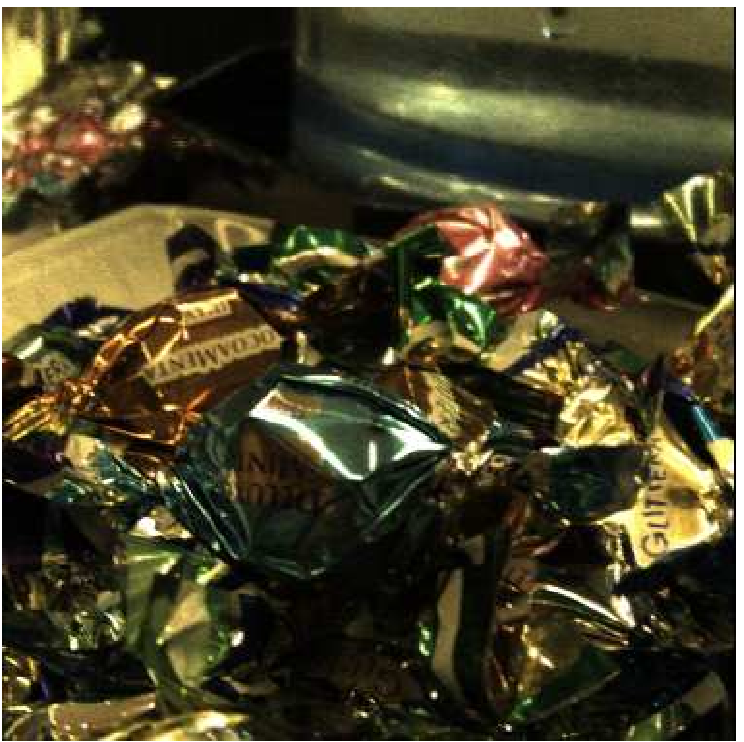
\includegraphics[width=0.32\textwidth]{Figs/Sample3}\\
	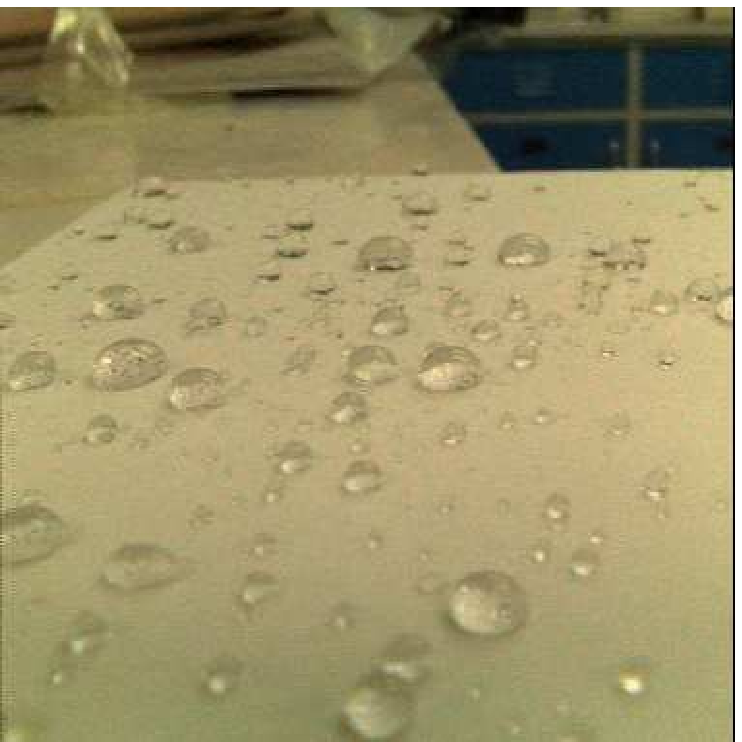
\includegraphics[width=0.32\textwidth]{Figs/Sample1_ColCorrect}
	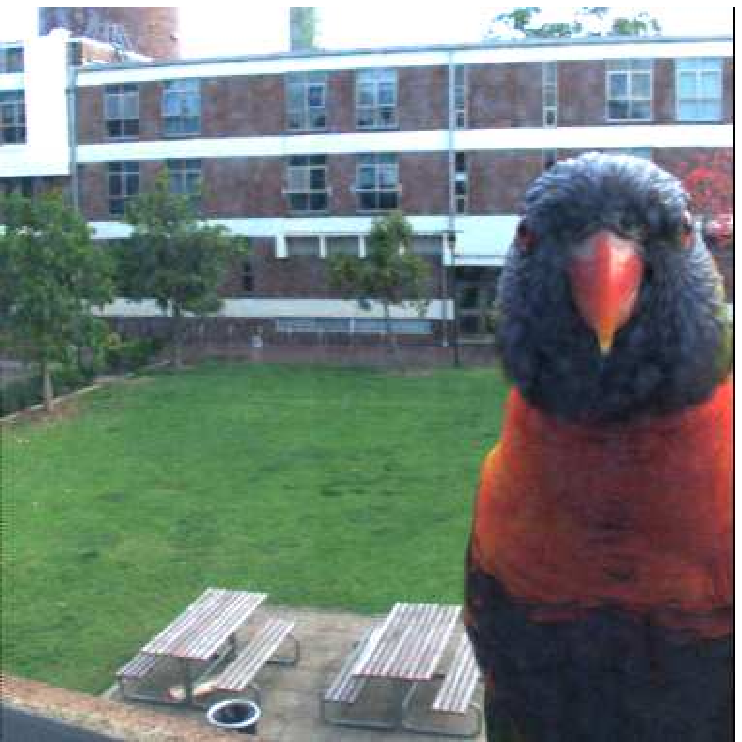
\includegraphics[width=0.32\textwidth]{Figs/Sample2_ColCorrect}
	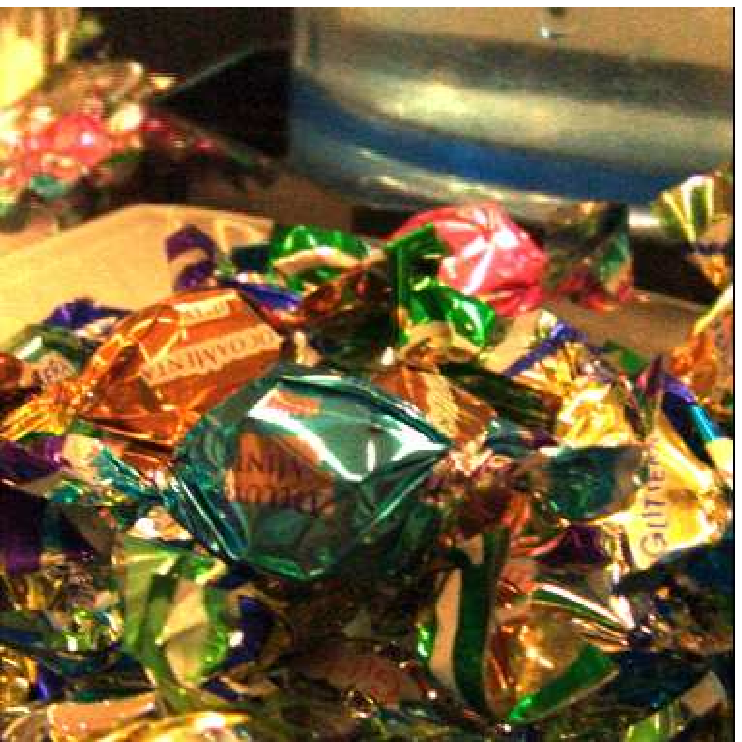
\includegraphics[width=0.32\textwidth]{Figs/Sample3_ColCorrect}
	\caption{Decoded (top) and colour-corrected output (bottom) -- the white speckles in the bird image are due to a pane of grubby glass between the camera and the bird. Running \protect\CiteFunc{LFDispVidCirc} or \protect\CiteFunc{LFDispMousePan} creates a shifting-perspective view in which this is more clear.}
	\label{fig_ExampleDecodeAndColourCorrectOutput}
\end{figure}

\begin{figure}[tbh]
	\centering
	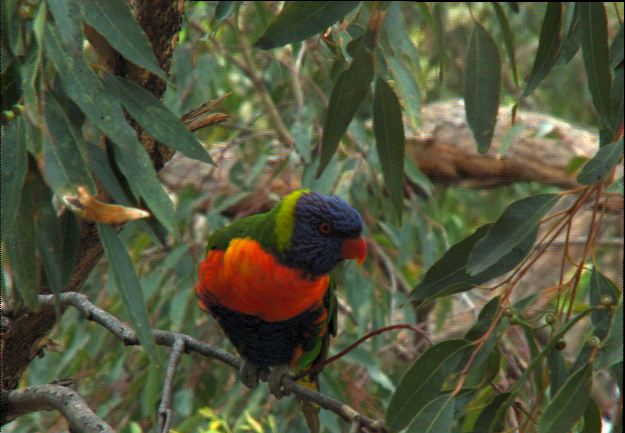
\includegraphics[width=0.49\textwidth]{Figs/IllumLorikeet1_adjusted}
	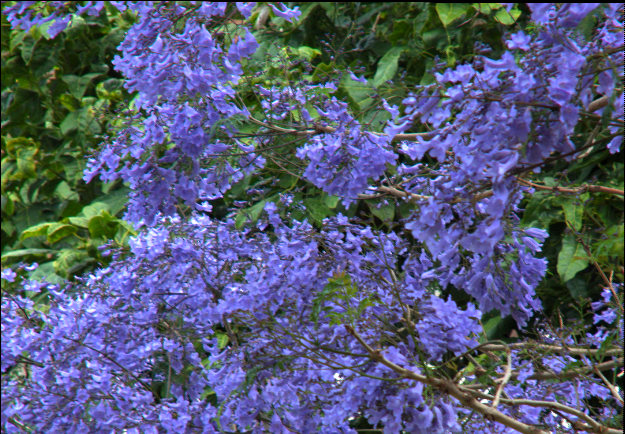
\includegraphics[width=0.49\textwidth]{Figs/IllumJacaranda_adjusted}
	\caption{Decoded and colour-corrected Illum images, manually Gamma-corrected by raising to the power 0.7.}
	\label{fig_ExampleIllumOutput}
\end{figure}


\item (optional) \textbf{Re-run \CiteFunc{LFUtilDecodeLytroFolder}} to perform colour correction. Use the commands
\begin{Verbatim}
DecodeOptions.OptionalTasks = 'ColourCorrect';
LFUtilDecodeLytroFolder([], [], DecodeOptions);
\end{Verbatim}

The \SymbolText{DecodeOptions} argument requests the optional task colour correction be performed. The first and second arguments are omitted by passing empty arrays \SymbolText{[]}.

Colour correction applies the information found in the light field metadata, including basic RGB colour and Gamma correction. The script keeps track of which operations have been applied to each light field, and so it will not repeat the decoding process, but will instead load each already-decoded light field, operate on it, and \emph{overwrite} it with the colour-corrected light field. Similarly, subsequent requests will not repeat the already-completed colour correction operation.

Decoding and colour-correction can be performed in one step by including the \SymbolText{ColourCorrect} task in the first call to \CiteFunc{LFUtilDecodeLytroFolder}.

You may wish to apply histogram stretching using \CiteFunc{LFHistEqualize}. Illum imagery is not gamma-corrected.  Example colour-corrected output is shown in the bottom row of Fig.~\ref{fig_ExampleDecodeAndColourCorrectOutput}, and in Fig.~\ref{fig_ExampleIllumOutput}.
\end{enumerate}

\subsubsection{Rectifying the Samples}

Still operating from the top level of the samples folder:
\begin{enumerate}[leftmargin=1.5em,rightmargin=0.5cm]
\item \textbf{Run \CiteFunc{LFUtilProcessCalibrations}} to locate and catalogue camera calibrations. The result is stored in \SymbolText{Cameras/CalibrationDatabase.mat}.
\item \textbf{Run \CiteFunc{LFUtilDecodeLytroFolder}} to rectify a specific light field:
\begin{Verbatim}
DecodeOptions.OptionalTasks = 'Rectify';
LFUtilDecodeLytroFolder( ...
    'Images/F01/IMG_0002__frame.raw', [], DecodeOptions);
\end{Verbatim}
\end{enumerate}

\begin{figure}[tbh]
	\centering
	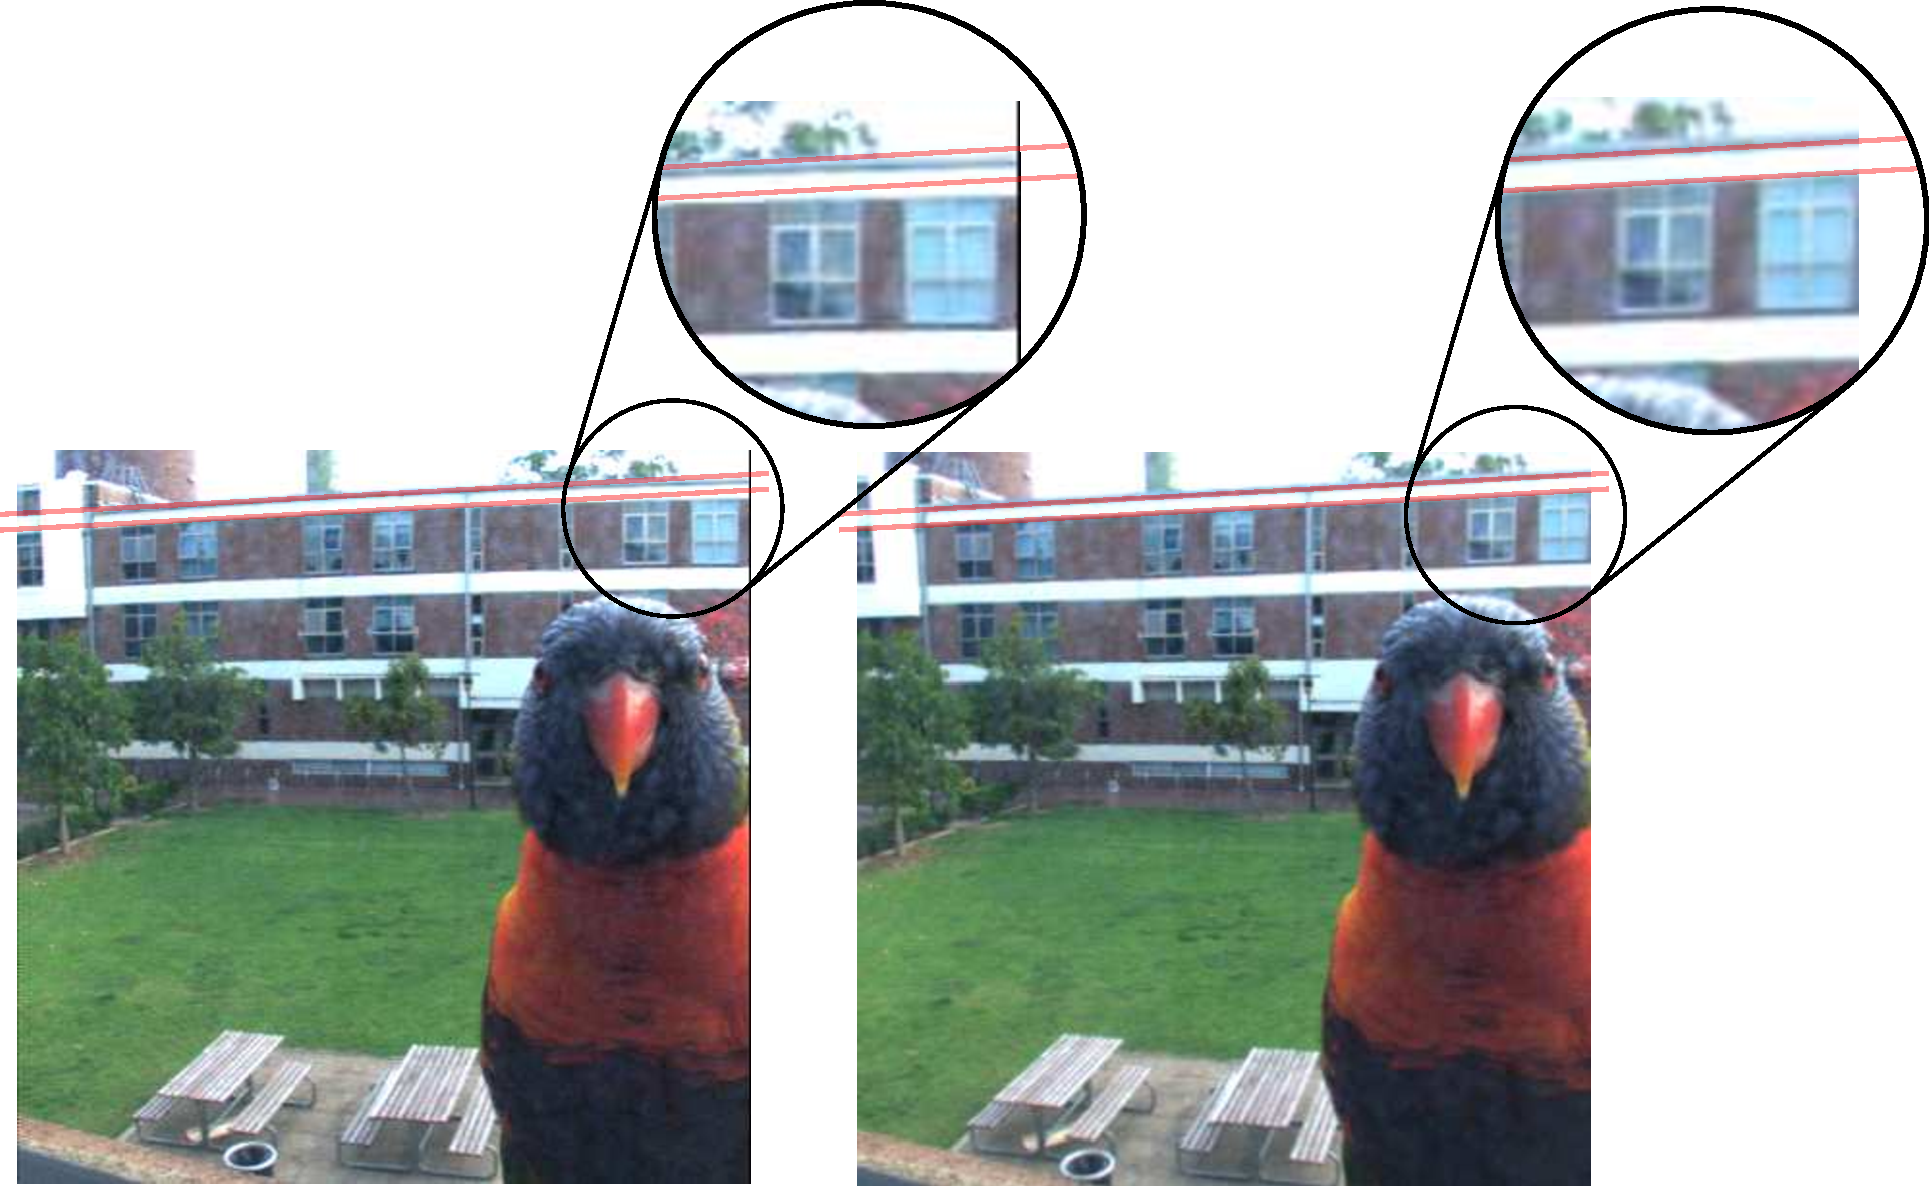
\includegraphics[width=1\textwidth]{Figs/Sample2_RectExample}
	\caption{F01 Sample 2 before and after rectification, with insets showing the reversal of lens distortion.}
	\label{fig_RectificationDetail}
\end{figure}

The \SymbolText{CalibrationDatabase} file allows selection of the calibration appropriate for each light field. Only one calibration is provided in the Sample Pack, and it is appropriate only for the F01 samples 2 and 5. 

As in the colour-correction example, we pass an \SymbolText{OptionalTasks} argument, this time requesting rectification. The rectified light field \emph{overwrites} the decoded light field file, and the decoding script will not repeat already-completed rectifications. The result of rectifying Sample 2 is shown in Fig.~\ref{fig_RectificationDetail}.

To rectify your own light fields, you must calibrate your camera.  See Sect.~\ref{sect_Calibration}.

\subsubsection{Using a Different Folder Structure}

You may wish to organize files differently than the toolbox default. A common use case is storing the \SymbolText{Camera} folder in a single global location outside the folder structure of the images.  The toolbox supports this via function parameters specifying file locations. For example, to decode images using a global camera folder:
\begin{Verbatim}
cd <top level path of your light field images>
DecodeOptions.WhiteImageDatabasePath = '<path to your cameras folder>';
LFUtilDecodeLytroFolder('.',[],DecodeOptions);
\end{Verbatim}
Note that you must still run \CiteFunc{LFUtilProcessWhiteImages} at the top level of your cameras folder. Use \SymbolText{RectOptions.CalibrationDatabaseFname} to specify the path to calibration files.

%----------------------------]-
\subsection{Displaying Light Fields}
\label{sect_DisplayingTour}
%-----------------------------
\begin{enumerate}[leftmargin=1.5em,rightmargin=0.5cm]
\item \textbf{Load} a light field, e.g.
\begin{Verbatim}
load('Images/Illum/Lorikeet__Decoded.mat','LF');
\end{Verbatim}
\item \textbf{Run \CiteFunc{LFDisp}} to display the central view of the light field.
\begin{Verbatim}
LFDisp( LF )
axis image    % for correct aspect ratio
\end{Verbatim}
To brighten the display through simple gamma correction, we can raise the light field to a power, but this first requires us to convert the light field to a floating point format first:
\begin{Verbatim}
LF = LFConvertToFloat(LF);
LFDisp( LF.^0.5 )
axis image
\end{Verbatim}
This is not very efficient, as it raises the entire light field to the power 0.5, then displays only the central view. You can use the following trick to nest LFDisp commands:
\begin{Verbatim}
LFDisp( LFDisp(LF).^0.5 )
axis image
\end{Verbatim}
This works because LFDisp returns the image as an output argument. The innermost LFDisp command extracts the central view of the light field, and only this view is then raised to 0.5. The result is passed to the outermost LFDisp for display. This approach can be applied with other display functions including \CiteFunc{LFHistEqualize}:
\begin{Verbatim}
LFDisp( LFHistEqualize(LFDisp(LF)).^0.5 )
axis image
\end{Verbatim}
\item \textbf{Run \CiteFunc{LFDispMousePan}, \CiteFunc{LFDispVidCirc}, or \CiteFunc{LFDispLawnmower}} to visualize the light field with a shifting perspective, e.g. 
\begin{Verbatim}
LFDispMousePan( LF )
\end{Verbatim}
\CiteFunc{LFDispMousePan} requires mouse input, click and drag in the window to change the perspective. The other functions animate through the images in the light field automatically.  Try a larger display with \SymbolText{LFDispMousePan(LF, 2)} or \SymbolText{LFDispVidCirc(LF, [], 2)}, which doubles the displayed size.

\item \textbf{Run \CiteFunc{LFDisp}} to display other slices of the light field:
\begin{Verbatim}
load('Images/Illum/Lorikeet__Decoded.mat','LF');
LFDisp( LF(9,:,226,:,:) );
\end{Verbatim}
displays a slice in $s,u$ at $t = 9$, $v = 226$. This is best viewed with a non-square aspect ratio by expanding the window horizontally.
\begin{Verbatim}
LFDisp( LFHistEqualize( LFDisp( LF(9,:,226,:,:) ) ).^0.7 )
\end{Verbatim}
displays the same contrast-stretched and gamma-corrected.

\item \textbf{Run \CiteFunc{LFDispTiles}} to visualize the light field as a 2D tiling of 2D images:
\begin{Verbatim}
load('Images/F01/IMG_0005__Decoded.mat','LF');
LFDispTiles(LF, 'stuv')
\end{Verbatim}
to display a tiling of $u,v$ slices in $s,t$. This is a large image, you can display a subset of the views using
\begin{Verbatim}
LFDispTiles( LF, 'stuv', struct('SubsampRate',2))
\end{Verbatim}
which will display every other sample in each of the four dimensions, or 
\begin{Verbatim}
LFDispTiles( LF(:,:, 85:100, 230:245, :) )
\end{Verbatim}
to display a crop in $u,v$. As with \CiteFunc{LFDisp}, \CiteFunc{LFDispTiles} returns the displayed image, allowing nesting:
\begin{Verbatim}
LFDisp( LFHistEqualize( LFDispTiles( LF(:,:,85:100, 230:245,:) ) ) )
\end{Verbatim}
stretches the contrast of the previous example.
\begin{Verbatim}
LFDispTiles( LF, 'uvst' )
axis image
\end{Verbatim}
will display a tiling of $s,t$ slices in $u,v$. Zoom in on the display to see individual lenslet images, or crop the light field when calling the display function, as in
\begin{Verbatim}
LFDispTiles( LF(:, :, 85:100, 230:245, :), 'uvst' )
\end{Verbatim}

\item \textbf{Run \CiteFunc{LFDispProj}} to visualize the light field as a projection onto a 2D plane
\begin{Verbatim}
load('Images/Illum/Lorikeet__Decoded.mat','LF');
LFDispProj( LF, 3,4 )
axis image
\end{Verbatim}
projects onto dimensions 3 and 4 ($v$ and $u$) by adding along the remaining dimensions, $s$ and $t$. The result is equivalent to refocus at the zero-slope depth.
\begin{Verbatim}
LFDispProj( LF, 3,4, 'max' )
axis image
\end{Verbatim}
does the same but finds the maximum value along $s,t$ for each $u,v$ sample, yielding an interesting effect.
\begin{Verbatim}
LFDispProj( LF, 1,2 )
axis image
\end{Verbatim}
projects onto the $s,t$ plane, revealing the lenslet vignetting pattern. It is mostly flat because it has been corrected in decoding.  The weight channel shows us a better picture of this:
\begin{Verbatim}
LFDispProj( LF(:,:,:,:,4), 1,2 )
colormap gray
axis image
\end{Verbatim}
We can also project onto $s,u$ or $t,v$ slices
\begin{Verbatim}
LFDispProj( LF, 2,4 )
axis normal
\end{Verbatim}
this is best viewed with a non-square aspect ratio by resizing the window. The contrast on this image is low since all the differently sloped parts of the scene are adding together. To get more of the structure apparent in the projection onto $s,u$, find the max along $s,v$ rather than the mean:
\begin{Verbatim}
LFDispProj( LF, 2,4, 'max' )
\end{Verbatim}

\end{enumerate}

%----------------------------]-
\subsection{Loading Gantry-style Light Fields}
\label{sect_LoadingGantryTour}
%-----------------------------

Camera gantries and camera arrays yield ordered collections of individual image files, with each image corresponding to a different aperture position. \CiteFunc{LFReadGantryArray} will read such an array of images as a light field.

\begin{enumerate}[leftmargin=1.5em,rightmargin=0.5cm]

\item \textbf{Download} an image archive from the Stanford gantry-based light field archive \url{http://lightfield.stanford.edu}, e.g.\ the LegoKnights light field.  Download the ``Rectified and cropped'' version.

\item \textbf{Unzip} the archive into a dedicated folder for Stanford samples. Following a structure like the following will allow \CiteFunc{LFDemoBasicFiltGantry} to run unmodified.

\NewAnnotatedTree{6}
\AnnotatedTreeEntry{0}{7}{StanfordGantry}{Top of Stanford gantry light fields}\\
\AnnotatedTreeEntry{1}{6}{JellyBeans}{}\\
\AnnotatedTreeEntry{2}{5}{rectified}{Rectified and cropped image files}\\
\AnnotatedTreeEntry{1}{6}{LegoKnights}{}\\
\AnnotatedTreeEntry{2}{5}{rectified}{Rectified and cropped image files}
\EndAnnotatedTree

\item \textbf{Run \CiteFunc{LFReadGantryArray}} from the top-level of the Stanford gantry samples:
\begin{Verbatim}
cd <path to top of Stanford gantry samples>
LF = LFReadGantryArray('LegoKnights/rectified', struct('UVLimit', 256));
\end{Verbatim}
The \SymbolText{UVLimit} option scales the images as they're read to a size of 256x256. By default \CiteFunc{LFReadGantryArray} looks for \SymbolText{.png} files, and assumes an array of 17 x 17 images in row major order. See the function help for specifying other filenames, array sizes, and file orderings.

\item \textbf{Run \SymbolText{size LF}} to check the light field size: \SymbolText{17 x 17 x 256 x 256 x 3}.

\item \textbf{Run \CiteFunc{LFDispMousePan}} or other display functions to display the loaded light field.

\end{enumerate}

It's possible to read the Stanford gantry light fields at full resolution, e.g.\ the following yields a 17 x 17 x 1024 x 1024 x 3 array, occupying 909 MBytes of RAM:
\begin{Verbatim}
LF = LFReadGantryArray('LegoKnights/rectified');
\end{Verbatim}
  
Some gantry imagery follows a lawnmower pattern rather than direct raster scan order.  These can be read and adjusted as follows:
\begin{Verbatim}
LF = LFReadGantryArray('humvee-tree', struct('STSize', [16,16]));
LF(1:2:end,:,:,:,:) = ...
  LF(1:2:end,end:-1:1,:,:,:);  % correct lawnmower ordering
\end{Verbatim}

Some gantry imagery follows a different handedness in horizontal and vertical directions, effectively flipping the order of images in $s$ or $t$.  The demo function \CiteFunc{LFDemoBasicFiltGantry} contains a list of Stanford gantry light fields and demonstrates how to flip the appropriate ones along $s$.

%----------------------------]-
\subsection{Working with ESLF Files}
\label{sect_ESLFTour}
%-----------------------------

Many of the large online datasets are stored as ESLF files. These collapse the light field into a 2D image by tiling $s,t$ slices in $u,v$. Because they are 2D images, they can be saved using any 2D image format. Popular choices are 8-bit and 16-bit \SymbolText{png} files for their lossless compression, and \SymbolText{jpg} files, for their compact size.  

\SymbolText{png} files support storage of an `alpha' channel, and some tools use this as a binary mask to indicate which pixels are valid. The toolbox can also save weight values in the alpha channel, indicating per-pixel confidence. By default, \CiteFunc{LFReadESLF} will load the alpha channel as a weight channel if it is present, but \CiteFunc{LFWriteESLF} will only write to the alpha channel if this is requested via the command arguments.

\subsubsection{Reading ESLF Files}

\begin{enumerate}[leftmargin=1.5em,rightmargin=0.5cm]

\item \textbf{\SymbolText{cd <sample folder>}} inside MATLAB to change to the top level of the samples folder.

\item \textbf{Run \CiteFunc{LFReadESLF}} to read the sample ESLF file:
\begin{Verbatim}
LF = LFReadESLF('Images/ESLF/Plant.eslf.jpg');
\end{Verbatim}

\item \textbf{Run \CiteFunc{LFDispMousePan}} to display the light field:
\begin{Verbatim}
LFDispMousePan(LF);
\end{Verbatim}

\item To load an ESLF file with a different number of pixels per lenslet, \textbf{Run \CiteFunc{LFReadESLF}} with the appropriate option, e.g. after writing \SymbolText{Jacaranda.eslf.png} in the next section, read it using
\begin{Verbatim}
LF = LFReadESLF('Jacaranda.eslf.png', [15,15]);
\end{Verbatim}
\end{enumerate}

\subsubsection{Writing ESLF Files}

\begin{enumerate}[leftmargin=1.5em,rightmargin=0.5cm]
\item Load a light field, and \textbf{Run \CiteFunc{LFWriteESLF}} to save it a PNG-compressed ESLF:
\begin{Verbatim}
load('Images/Illum/Jacaranda__Decoded.mat','LF');
WriteAlpha = true;
LFWriteESLF( LF, 'Jacaranda.eslf.png', WriteAlpha );
\end{Verbatim}
Because the loaded light field is 16-bit and has a weight channel, and we requested the alpha channel be written, the output \SymbolText{png} is 16-bit and has four channels, occupying 418~MBytes. If we do not request the alpha channel be written, 
\begin{Verbatim}
LFWriteESLF( LF, 'Jacaranda.eslf.png' );
\end{Verbatim}
the file occupies 300~MBytes. If we first convert to 8-bit pixels using \CiteFunc{LFConvertToInt} and omit the alpha channel, 
\begin{Verbatim}
LF = LFConvertToInt( LF, 'uint8' );
LFWriteESLF( LF, 'Jacaranda.eslf.png' );
\end{Verbatim}
the file occupies 102~MBytes. 

\item After converting the light field to 8-bit format as above, \textbf{Run \CiteFunc{LFWriteESLF}} to save a ligt field as a JPEG-compressed ESLF:
\begin{Verbatim}
LFWriteESLF( LF, 'Jacaranda.eslf.jpg' );
\end{Verbatim}
The resulting 8-bit lossily compressed light field without a weight channel occupies only 16~MBytes, but upon loading and displaying it you may notice strong compression artefacts. Adjust the JPEG compression rate to increase quality
\begin{Verbatim}
LFWriteESLF( LF, 'Jacaranda.eslf.jpg', [], 'Quality', 95 );
\end{Verbatim}
looks significantly better and occupies 38~MBytes.
\end{enumerate}

%-----------------------------
\subsection{Basic Filters}
%-----------------------------

\begin{figure}
	\centering
	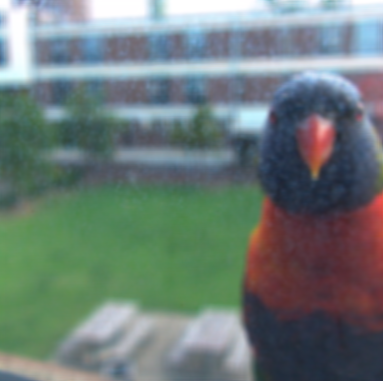
\includegraphics[width=0.32\textwidth]{Figs/Sample2_ShiftSumWindow}
	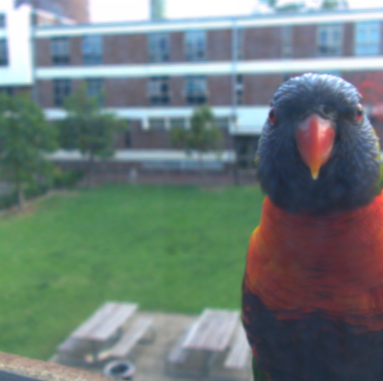
\includegraphics[width=0.32\textwidth]{Figs/Sample2_ShiftSumLorikeet}
	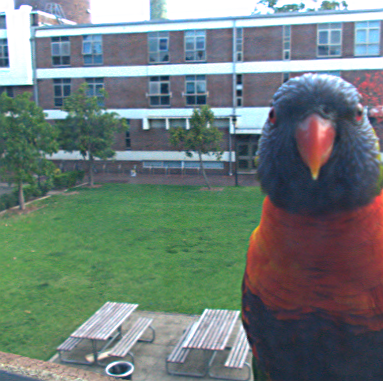
\includegraphics[width=0.32\textwidth]{Figs/Sample2_HyperfanNoWindow}
	\caption{Three examples of filtering Lytro imagery: the shift-and-sum filter performing planar focus on the foreground window (left) and on the Lorikeet (center), and a hyperfan filter performing volumetric focus to pass the Lorikeet and background building while rejecting the foreground window (right, compare with Fig.~\ref{fig_ExampleDecodeAndColourCorrectOutput}).}
	\label{fig_ExampleFilterOutputLytro}
\end{figure}

\begin{figure}
	\centering
	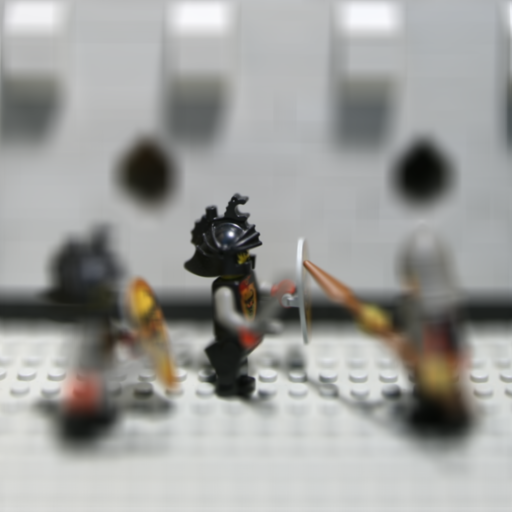
\includegraphics[width=0.32\textwidth]{Figs/Lego512_ShiftSum_n0.6}
	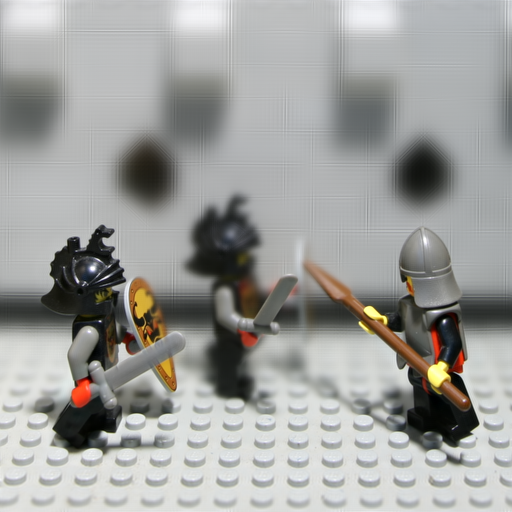
\includegraphics[width=0.32\textwidth]{Figs/Lego512_Hyperfan_n0.6_2}
	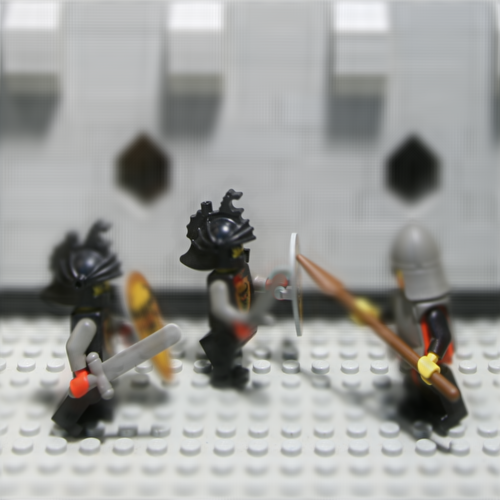
\includegraphics[width=0.32\textwidth]{Figs/Lego512_Hyperfan_n0.8_0.8}
	\caption{Three examples of filtering gantry imagery: the shift-and-sum filter performing planar focus (left), the hyperfan filter performing volumetric focus (center), and the max between two hyperfan filters, focusing simultaneously on two planes (right).}
	\label{fig_ExampleFilterOutputGantry}
\end{figure}

\begin{figure}
	\centering
	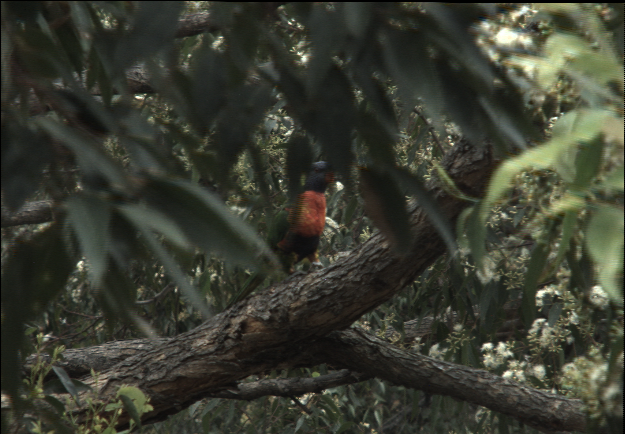
\includegraphics[width=0.49\textwidth]{Figs/LorikeetHiding_in}
	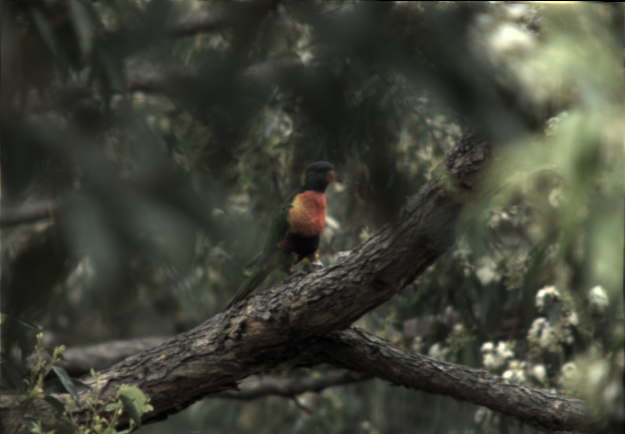
\includegraphics[width=0.49\textwidth]{Figs/LorikeetHiding_shiftsum_bird}
	\caption{Examples of filtering Lytro Illum imagery, showing the input (left) and shift-and-sum filter performing planar focus (right).}
	\label{fig_ExampleFilterOutputIllum}
\end{figure}

The toolbox comes with a spatial shift-and-sum filter for planar focus and refocus super-resolution, and a set of linear 2D and 4D filters for planar and volumetric focus.

Run one of \CiteFunc{LFDemoBasicFiltLytroF01} or \CiteFunc{LFDemoBasicFiltIllum} for a demo of some of the filters operating on Lytro imagery. This should be done from the top level of the Samples folder, after decoding the light fields as described in Sect.~\ref{sect_DecodingLytro}.  The best performance is obtained with rectified light fields.

Run \CiteFunc{LFDemoBasicFiltGantry} for a demo filtering the Stanford gantry light fields.  This should be done from the top of the Stanford gantry light fields folder, after downloading and unzipping the samples following the instructions in Sect.~\ref{sect_LoadingGantryTour}. Uncomment the appropriate line near the top of \CiteFunc{LFDemoBasicFiltGantry} to select from the 12 input light fields.

Examples of filtering output are shown in Figs.~\ref{fig_ExampleFilterOutputLytro}, \ref{fig_ExampleFilterOutputGantry}, and~\ref{fig_ExampleFilterOutputIllum}.


\subsubsection{Linear Refocus Super-Resolution}
\label{sect_SuperResTour}
New in v0.5 is linear refocus super-resolution. This is a way to simultaneously focus at a single depth and boost the resolution of the result. The method modifies \CiteFunc{LFFiltShiftSum} to upsample each image prior to shifting, effectively allowing fractional shifts, and boosting resolution in the merged image. 

Note that this approach only adds information for fractional slopes, images focused at integer slopes will see no benefit. Note also that the upsampling ratio does not reflect the effective resolution increase: upsampling by $10 \times$ might only increase effective resolution by $1.5 - 2 \times$, for example.

Typical results are shown in Fig.~\ref{fig_RefocusSuperResolution}, for an upsampling rate of $10 \times$. These are tight crops on the Flowers sample ESLF and \SymbolText{IMG\_6201.eslf.png} from the Flowers category of the Stanford Multi-View Light Field dataset at \url{http://lightfields.stanford.edu}.

From the figure, we clearly see a dramatic improvement in the visual appearance of the `Super-res' result compared with the `Focus' result. Comparing with `2D Interp' cubic interpolation, we see a less dramatic but still noticeable improvement more representative of the effective resolution increase offered by this approach. Better camera calibration and light field rectification will increase the effectiveness of this form of super-resolution.

For a demonstration of linear refocus super-resolution, see \CiteFunc{LFDemoRefocusSuperres}.

\begin{figure}[tbh]
	\centering
	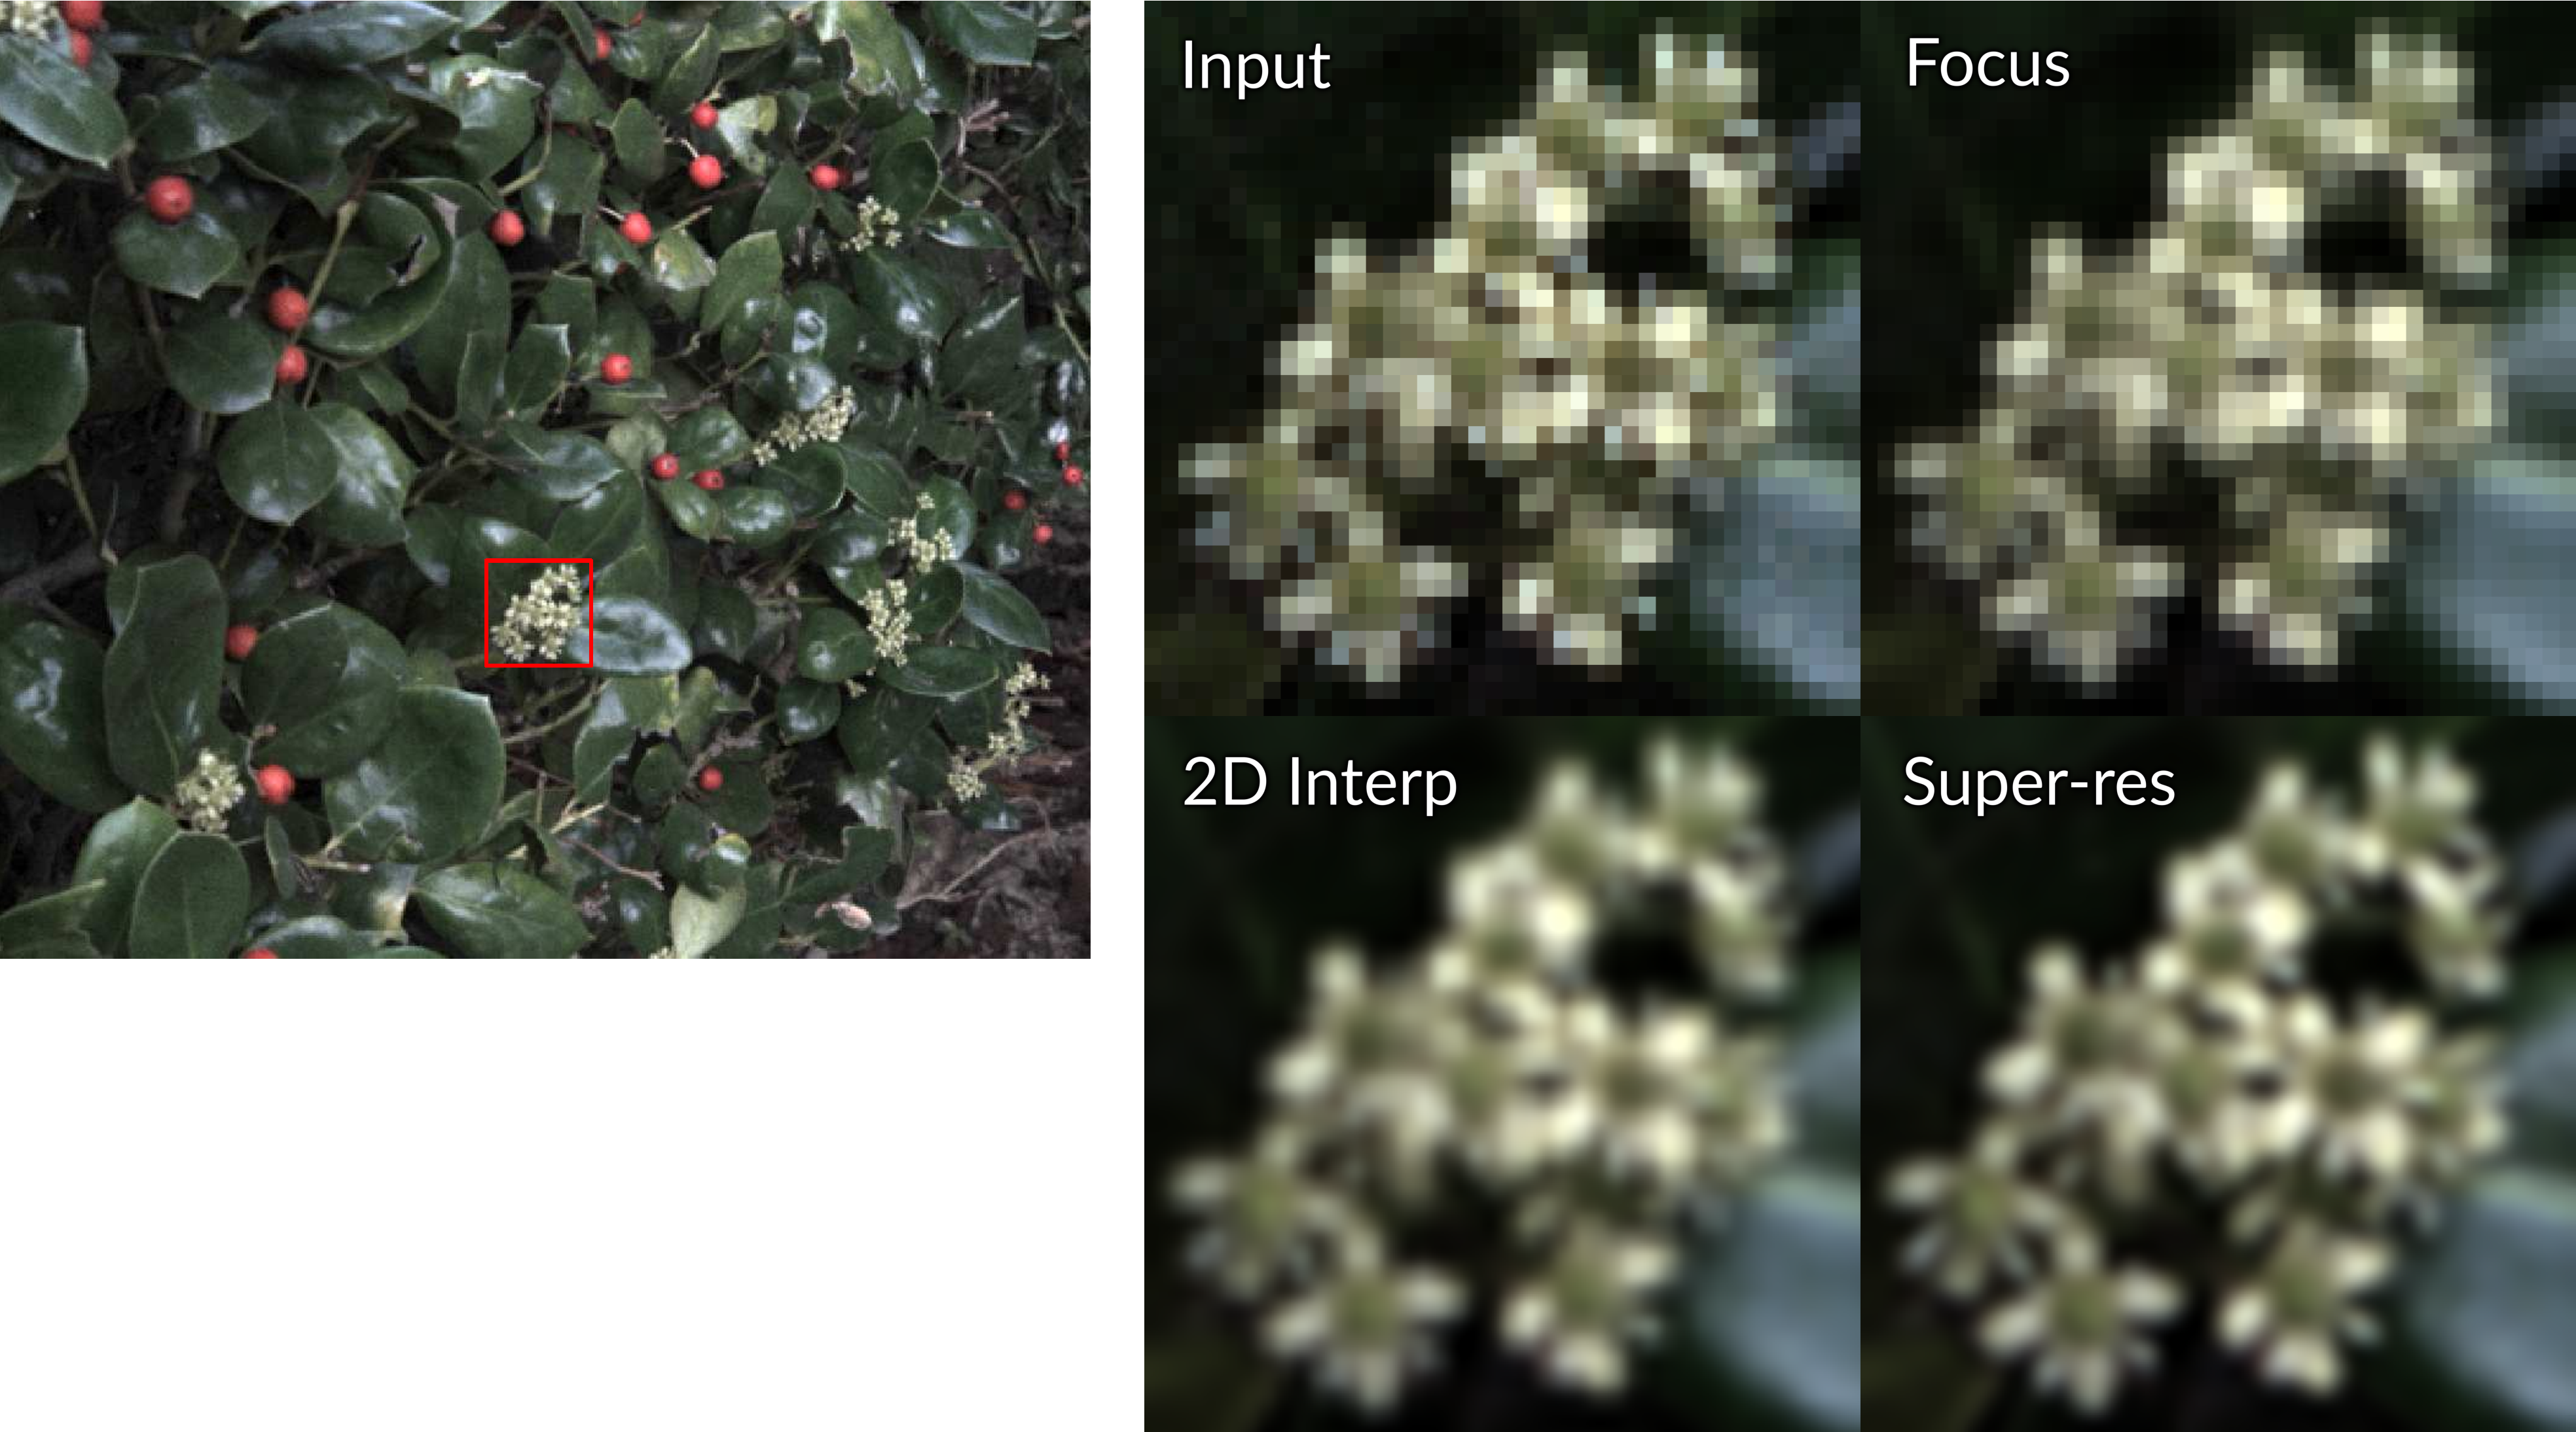
\includegraphics[width=1\textwidth]{Figs/RefocusSuperRes}
	\caption{Linear super-resolution using \protect\CiteFunc{LFFiltShiftSum}. The inputs are small crops from larger light fields; `Focus' shows focus alone, mostly removing noise and limiting depth of field; '2D Interp' shows 2D cubic interpolation applied to the focus image, for comparison; and `Super-res' shows linear super-resolution with noticeably finer detail than focus alone or 2D interpolation. See \protect\CiteFunc{LFDemoRefocusSuperres} for usage.}
	\label{fig_RefocusSuperResolution}
\end{figure}


%-----------------------------
\subsection{Running the Small Sample Calibration}
%-----------------------------
\subsubsection{Calibrating}
%-----------------------------

The example below assumes you've completed the Decoding tour above, including generating the white image database. The small calibration dataset employed here is intended only to quickly demonstrate operation of the toolbox, and has several shortcomings in terms of effectively calibrating the camera:

\begin{itemize}
\item The checkerboard is too large for sufficiently short-range poses -- a lenslet-based camera has a small spatial baseline, and calibrating this baseline benefits from close-up poses
\item The checkerboard is not very dense -- more corners would be appropriate
\item There is insufficient diversity in the checkerboard poses -- ten or more diverse images would be appropriate
\end{itemize}

More realistic (and larger) datasets are available at \url{http://dgd.vision/Tools/LFToolbox}. Good results have been obtained using a $19 \times 19$ grid with a 3.6~mm spacing, with at least ten diverse poses.


\begin{figure}[tbh]
	\centering
	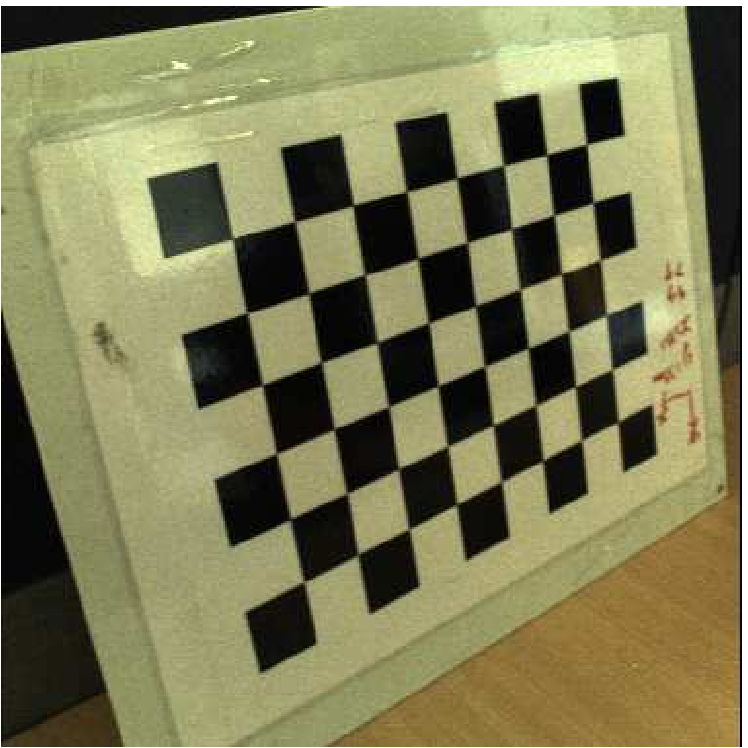
\includegraphics[width=0.48\textwidth]{Figs/CheckerboardExample}
	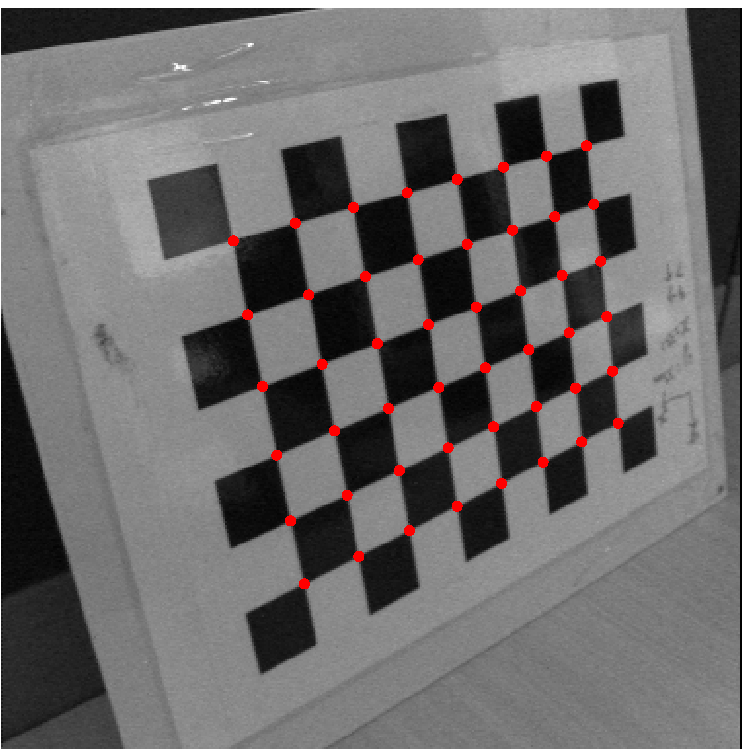
\includegraphics[width=0.48\textwidth]{Figs/CheckerboardMatchingExample}
	\caption{Left: Example of a decoded checkerboard image -- no colour correction is necessary and rectification should not be applied; Right: Example of checkerboard corners automatically fit to the checkerboard in the first step of a calibration.}
	\label{fig_CheckerboardAndCorners}
\end{figure}

\begin{enumerate}[leftmargin=1.5em,rightmargin=0.5cm]

\item \textbf{Download} the small sample calibration from \url{http://www-personal.acfr.usyd.edu.au/ddan1654/PlenCalSmallExample.zip}.  \textbf{Decompress to your \SymbolText{Samples/Cameras/A000424242/} folder}:

\NewAnnotatedTree{6}
\AnnotatedTreeEntry{0}{7}{Samples}{Top level of samples}\\
\AnnotatedTreeEntry{1}{6}{Cameras}{Stores info for one or more cameras}\\
\AnnotatedTreeEntry{2}{5}{A000424242}{The camera used to measure the samples}\\
\AnnotatedTreeEntry{3}{4}{CalZoomedOutFixedFoc}{A single calibration result}\\
\AnnotatedTreeEntry{3}{4}{\normalsize{\textbf{PlenCalSmallExample}}}{\textbf{The newly-added calibration}}\\
\AnnotatedTreeEntry{3}{4}{WhiteImages}{White images for the sample camera}\\
\AnnotatedTreeEntry{1}{6}{Images}{Sample light field images}\\
\EndAnnotatedTree

\item \textbf{Run \CiteFunc{LFUtilDecodeLytroFolder}} to decode the calibration light fields.  From within Matlab \SymbolText{cd} into the top level of the samples folder, then use the command
\begin{Verbatim}
LFUtilDecodeLytroFolder( ... 
     'Cameras/A000424242/PlenCalSmallExample/');
\end{Verbatim}

This should find and decode the calibration checkerboard images.  Note that colour-correction is omitted as it is not required, and rectification would invalidate the results.  A thumbnail of one of the decoded checkerboard images is shown in Fig.~\ref{fig_CheckerboardAndCorners}.

\item \textbf{Run \CiteFunc{LFUtilCalLensletCam}} to run the calibration. This function automatically progresses through all the stages of calibration. Use the commands
\begin{Verbatim}
CalOptions.ExpectedCheckerSize = [8,6];
CalOptions.ExpectedCheckerSpacing_m = 1e-3*[35.1, 35.0];
LFUtilCalLensletCam( ...
    'Cameras/A000424242/PlenCalSmallExample', CalOptions);
\end{Verbatim}

These options tell the calibration function that the checkerboard spacing is $35.1 \times 35.0$ mm, and that there are $8 \times 6$ corners.  Note that edge corners are not included in this count, so a standard $8 \times 8$ square chess board yields $7 \times 7$ corners. These values are available in the README file that came with the calibration sample.  Calibration automatically proceeds through corner identification, parameter initialization, parameter optimization without lens distortion, then with lens distortion, and a final stage of parameter refinement.  These are described in more detail in Sect.~\ref{sect_Calibration}.

\begin{figure}[tbh]
	\centering
	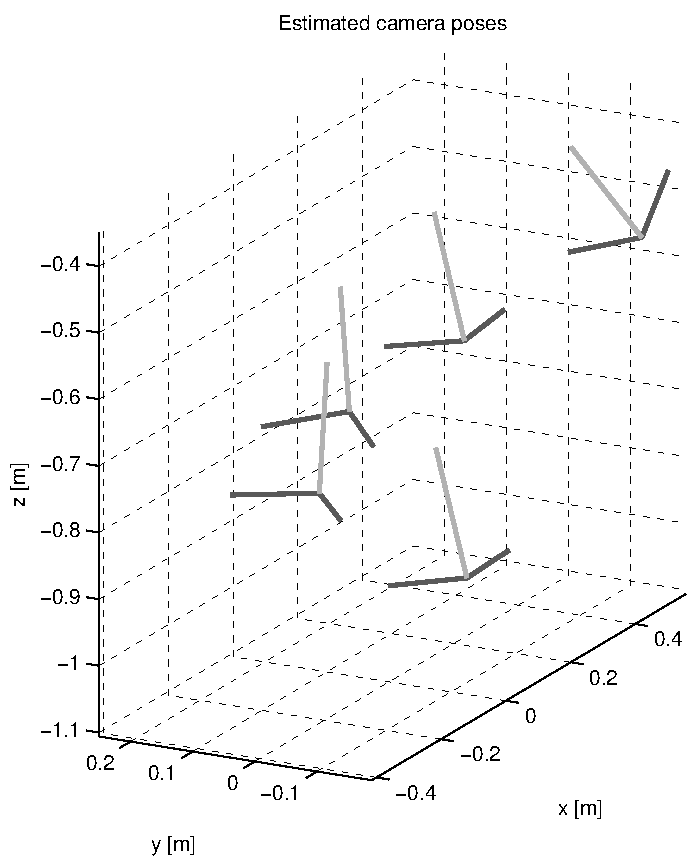
\includegraphics[width=0.48\textwidth]{Figs/SampleCalibrationPoseEstimates_InitOnly}
	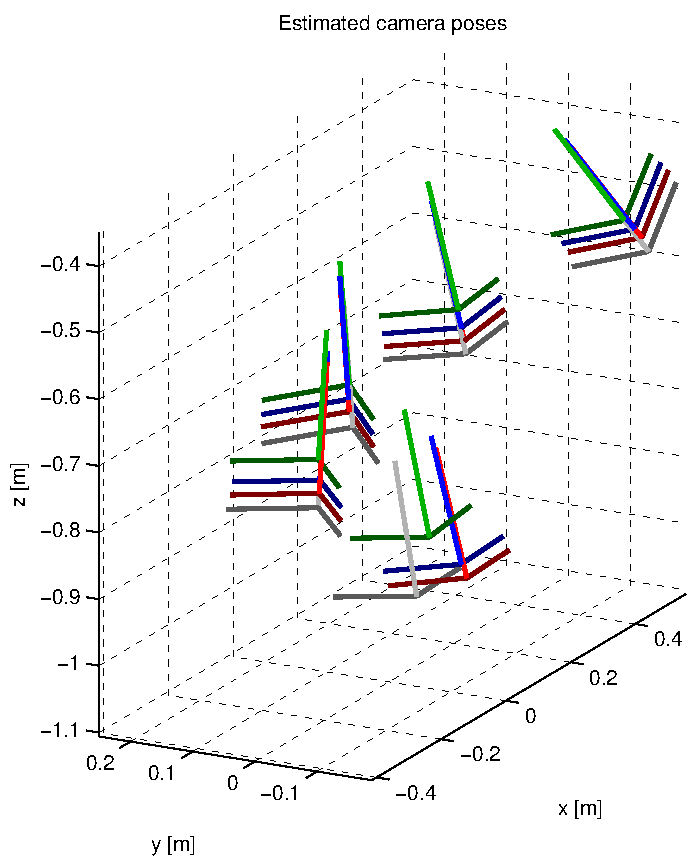
\includegraphics[width=0.48\textwidth]{Figs/SampleCalibrationPoseEstimates}
	\caption{The estimated camera pose display; Left: After parameter initialization, and Right: After completion of a calibration; Gray: initial estimate, Green: optimized without distortion, Blue: optimized with distortion, and Red: after refinement.}
	\label{fig_SampleCalibrationPoseEstimates}
\end{figure}

During the parameter initialization step, a pose estimate display is drawn resembling that shown in  Fig.~\ref{fig_SampleCalibrationPoseEstimates}. This display is updated throughout the remaining stages, reflecting the refinement of the pose and camera model estimates.  Reprojection errors are also shown in the text output.  Typical final root mean squared error (RMSE) values for the small calibration example are in the vicinity of 0.2~mm. 

The ultimate product of the calibration process is the calibration information file, \SymbolText{CalInfo.json}, which contains pose, intrinsic and distortion parameters, as well as the lenslet grid model used to decode the checkerboard light fields.

\end{enumerate}

%--------------------------
\subsubsection{Validating}

One way of validate a calibration is to rectify the checkerboard images. The process closely resembles the rectification step described in the Decoding tour:

\begin{enumerate}[leftmargin=1.5em,rightmargin=0.5cm]

\item \textbf{Run \CiteFunc{LFUtilProcessCalibrations}} to add the newly-completed calibration to the calibration database.  Note from the output of that function that the small calibration example is very close to the sample calibration provided with the sample pack, differing only by a few focus steps.

\item \textbf{Copy} all the files from \SymbolText{Cameras/A000424242/PlenCalSmallExample/01} into a new folder, \SymbolText{Samples/Images/PlenCalSmallExample}. This will allow rectification of the images while maintaining the unrectified versions for comparison.

\item \textbf{Run \CiteFunc{LFUtilDecodeLytroFolder}} to rectify the images.  Use the command
\begin{Verbatim}
DecodeOptions.OptionalTasks = 'Rectify';
LFUtilDecodeLytroFolder('Images/PlenCalSmallExample', ...
    [], DecodeOptions);
\end{Verbatim}

Examining the text output, notice that the rectification has automatically selected the small sample calibration for these images, based on their zoom and focus settings.

A visual inspection of the rectified images probably shows poor results, due to the limitations of the small calibration dataset.  When calibrating with your own camera, rectification should ideally show good results.

\end{enumerate}

%--------------------------
\subsubsection{Cleaning Up and Validating}

As discussed earlier in this section, the \SymbolText{CalInfo.json} generated from the small sample calibration is not very good.  When finished with the sample calibration, you should remove this file from\\ \SymbolText{Cameras/A000424242/PlenCalSmallExample} and re-run \CiteFunc{LFUtilProcessCalibrations}. Repeating the above validation procedure with the better, default sample calibration in place yields more reasonable validation results, such as those shown in Fig.~\ref{fig_CalibrationExampleRectification}, even despite a slight mismatch in camera parameters.

\begin{figure}[tbh]
	\centering
	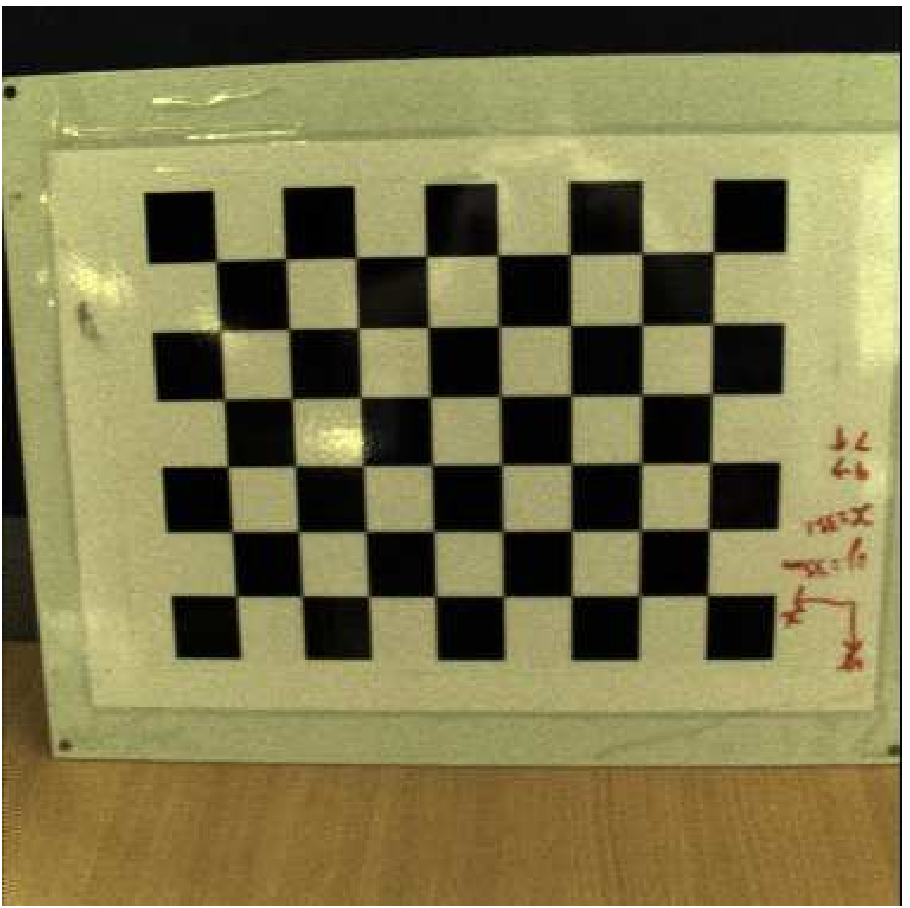
\includegraphics[width=0.48\textwidth]{Figs/SampleCalibrationRectIn}
	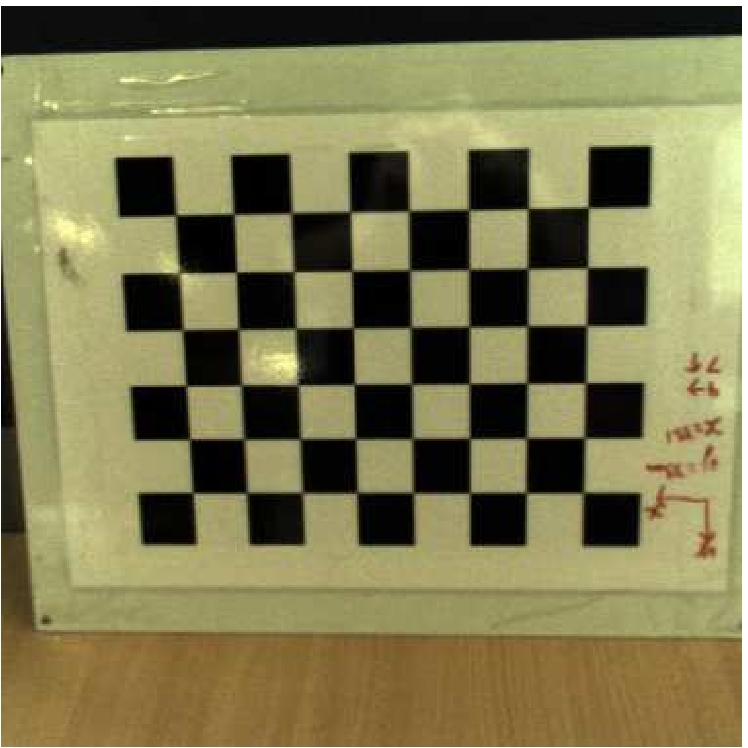
\includegraphics[width=0.48\textwidth]{Figs/SampleCalibrationRectOut}
	\caption{A rectified checkerboard; Run Fig.~\ref{fig_RectificationDetail}. More complete datasets are explored in [1].}
	\label{fig_CalibrationExampleRectification}
\end{figure}


%-----------------------------
\subsection{Beyond the Samples:\\Working with Your Own Light Fields}
%-----------------------------

Processing images from your own camera closely mirrors the examples covered so far.  First, create a new folder parallel to the \SymbolText{Cameras/A000424242} folder, to contain your camera's white images and any calibrations you perform. A good convention is to name this folder to match your camera's serial number.  Next, create a sub-folder for your white images. Your tree structure should now look like:

\NewAnnotatedTree{6}
\AnnotatedTreeEntry{0}{7}{Samples}{Top level of samples}\\
\AnnotatedTreeEntry{1}{6}{Cameras}{Stores info for one or more cameras}\\
\AnnotatedTreeEntry{2}{5}{\normalsize{A123412123}}{\textbf{Your camera's top level folder}}\\
\AnnotatedTreeEntry{3}{4}{\normalsize{WhiteImages}}{\textbf{Your camera's white images}}\\
\AnnotatedTreeEntry{2}{5}{A000424242}{The camera used to measure the samples}\\
\AnnotatedTreeEntry{3}{4}{CalZoomedOutFixedFoc}{A single calibration result}\\
\AnnotatedTreeEntry{3}{4}{WhiteImages}{White images for the sample camera}\\
\AnnotatedTreeEntry{1}{6}{Images}{Sample light field images}\\
\EndAnnotatedTree

Following the procedure described in Appendix~\ref{sect_LytroFiles}, extract your camera's white images and place them in the newly created \SymbolText{WhiteImages} folder.  Any calibrations you perform should sit in their own folders alongside the WhiteImages folder.

From the top level of the samples folder, run \CiteFunc{LFUtilProcessWhiteImages} to process your camera's white images.  The resulting grid models  will be added to the white image database, and automatically applied to pictures taken with your camera.

You may end up with a complex tree structure with many sub-folders under \SymbolText{Images}.  \CiteFunc{LFUtilProcessWhiteImages} will search this structure recursively, decoding anything it identifies as a light field.

To rectify your own images, you will need to calibrate your camera.  Follow the procedure described in the tour above, except using your own images stored within your own camera's folder.  Your first calibrations might, for example, go in \SymbolText{Samples/A123412123/CalZoomedOut}.


\subsection{Calibrating the Illum}

Calibration for the Lytro Illum remains experimental, and the toolbox can struggle for certain focal lengths.  Samples near the edges of lenslets are especially challenging, and short focal lengths (with the camera zoomed out) are also more challenging. To make things easier for calibration, try calibrating with the lens zoomed in somewhat, and increasing \SymbolText{CalOptions.LensletBorderSize} to 2 or 3 pixels. Future toolbox versions will address this shortcoming.


%-----------------------------
\section{Decoding in Detail}
\label{sect_DecodingInDetail}
%-----------------------------

The toolbox decodes lenslet-based light field images into a 4D light field structure following the process described in [1]. At its core, the inputs to this process are a white image and a lenslet image. 

The white image is a flat-field image that reveals the vignetting pattern of the camera, the darkening near the edges of images and lenslets.  White images are measured by taking an image of an evenly-illuminated white surface, by taking an image through a diffuser, or by using a specialized tool like an internally illuminated integrating sphere. The toolbox uses these images to correct for vignetting and to build a grid representing the locations of lenslet centers.

Each Lytro camera comes preloaded with a unique set of white images corresponding to a variety of zoom and focus settings. When decoding a light field picture, the white image is selected which most closely matches the zoom and focus settings of the camera when it took the picture. The white images can be extracted from the Lytro files following the instructions in Sect.~\ref{sect_LytroFiles_Cal}.

Before decoding light field pictures, the white images must be analyzed. This builds a series of grid models, one per white image, and a database listing available images. This only needs to be done once per camera, and the utility function \CiteFunc{LFUtilProcessWhiteImages} automates the process.

For each picture to decode, a white image appropriate to that picture is selected based on the camera serial number and zoom and focus settings. The white image and raw lenslet image are passed to a decoding function which builds the 4D light field. The function \SupFunction{LFSelectFromDatabase} selects the appropriate white image for a light field, and is used by \CiteFunc{LFLytroDecodeImage}.

The following sections describe this workflow in more detail, and assumes that you have extracted the white images and copied light fields into a folder structure similar to that used in the quick tour, above. See Appendix~\ref{sect_LytroFiles} for details on dealing with the Lytro files.

%-----------------------------
\subsection{Analyzing White Images}
\label{sect_AnalyzingWhiteImages}
Each white image needs to be analyzed once in order to match a grid model to the lenslet locations. The utility \CiteFunc{LFUtilProcessWhiteImages} builds a grid model for each white image in your white image folder. If you wish to store your white images in a structure other than the default, change the \SymbolText{WhiteImageDatabasePath} variable in \CiteFunc{LFUtilProcessWhiteImages} to point to your white images folder, or use the function argument \SymbolText{FileOptions.WhiteImageDatabasePath}.

In the F01 camera, the white images come in two exposure levels. Only the brighter of the two is used by this toolbox. The set of white images also generally includes some very dark images. These are not ignored by the toolbox.

As \CiteFunc{LFUtilProcessWhiteImages} steps through the white images, it saves the grid models as \SymbolText{.grid.json} files in the white images folder. It simultaneously builds a database keeping track of the serial number, zoom and focus settings associated with each white image. It saves this as \SymbolText{WhiteFileDatabase.mat}.  This is utilized by the function \SupFunction{LFSelectFromDatabase} to select the white image appropriate for decoding a given light field picture.

%-----------------------------
\subsection{Decoding a Lenslet Image}

The decode procedure is demonstrated in \CiteFunc{LFLytroDecodeImage}. This script first loads a lenslet image and associated metadata, selects the appropriate white image using \SupFunction{LFSelectFromDatabase}, then passes the lenslet image, metadata and white image to \SupFunction{LFDecodeLensletImageSimple}, which handles the bulk of the work.

\SupFunction{LFSelectFromDatabase} selects the appropriate white image based on serial number, zoom and focus settings. Presently zoom is prioritized over focus, though whether this is the optimal approach is an open question.

\SupFunction{LFDecodeLensletImageSimple} proceeds as described in [1] to decode the light field. This involves demosaicing, devignetting, transforming and slicing the input lenslet image to yield a 4D structure. More sophisticated approaches exist which combine steps into joint solutions, and they generally yield superior results, particularly near the edges of lenslets. The approach taken here was chosen for its simplicity and flexibility.

Some of the specifics of the decode process can be controlled, see the help text for the above functions.

%-----------------------------
\subsection{Structure of the Decoded Light Field}

A light field is fundamentally a four-dimensional structure. Roughly speaking, each pixel corresponds to a ray, and two dimensions define that ray's position, while the other two define its direction. In the case of the the images measured by a lenslet-based camera such as the Lytro, two dimensions select a lenslet image, and two select a pixel within that lenslet's image. By the convention followed in [1], the lenslet is indexed by the pair $k, l$ ($k$ is horizontal), and the pixel within the lenslet is indexed by $i, j$ ($i$ is horizontal). When it is clear that discrete indices are being discussed, these are often referred to using their continuous-domain equivalents, $s,t$ for $i,j$, and $u,v$ for $k,l$.

The Lytro F01's lenslets each yield approximately $9 \times 9$ useful pixels, and so the output of \CiteFunc{LFUtilDecodeLytroFolder} has a size approximately 9 in $i$ and $j$. Similarly, after removing the hexagonal sampling associated with the hexagonal lenslet array, the Lytro imagery yields approximately $380$ pixels in both $k$ and $l$.  The Illum has more lenslets and more pixels per lenslet. The actual number of samples in a light field depends on how the lenslet grid is aligned with the sensor, and can vary by a few samples between cameras.

Examining the output of \SupFunction{LFDecodeLensletImageSimple}, we see that it yields a light field \SymbolText{LF} which is a 5D array of size around $9\times9\times380\times380\times3$. As discussed in Sect.~\ref{sect_Conventions}, \textbf{the indexing order for \SymbolText{LF} is $j, i, l, k, c$}, where c is the RGB colour channel. 

\begin{figure}[tbh]
	\centering
	
\includegraphics[height=0.45\textwidth]{Figs/STSlice}
	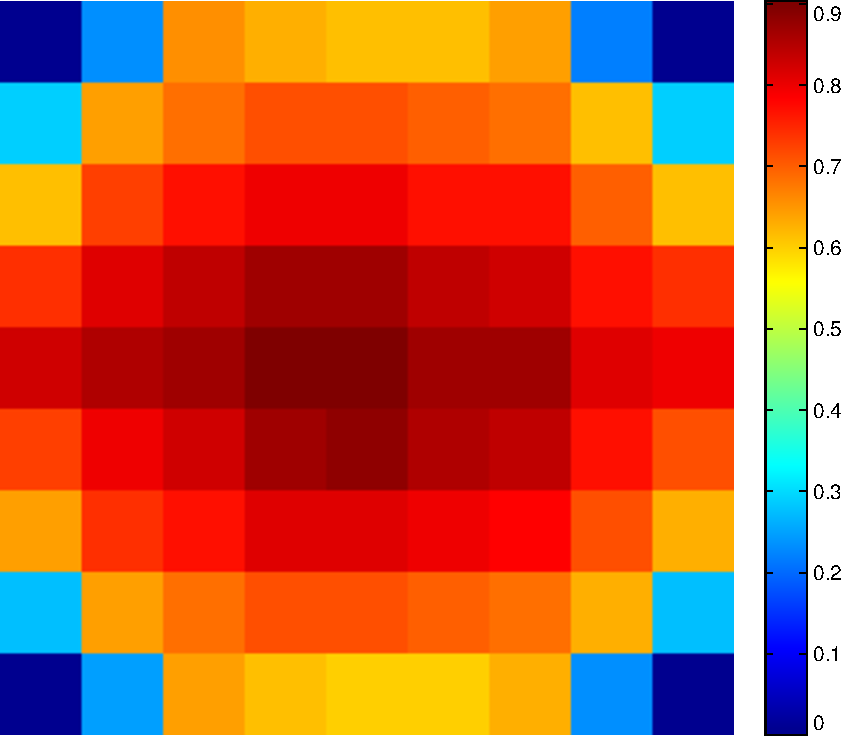
\includegraphics[height=0.45\textwidth]{Figs/WeightSTSlice}
	\caption{Light field for Sample 1 and its associated weight channel viewed in the $i$ and $j$ dimensions.}
	\label{fig_STSlice}
\end{figure}

To examine a slice through the $k$ and $l$ dimensions, you might use the command \SymbolText{imshow(squeeze(LF(5,5,:,:,:)))}, yielding a view from the center of the $i$ and $j$ dimensions similar to the output of \SymbolText{LFDisp(LF)}. To examine a slice through the $i$ and $j$ dimensions, you might use the command \SymbolText{imshow(squeeze(LF(:,:,380/2,380/2,:)))}, with an output similar to that shown in Fig.~\ref{fig_STSlice}. Notice this shows the shape of the image under a lenslet, with darkened corner pixels that contain little or no information. See Sect.~\ref{sect_DisplayingTour} for more ways of displaying light fields.

\SupFunction{LFDecodeLensletImageSimple} provides a weight channel \SymbolText{LFWeight}, which represents the confidence associated with each pixel. A slice in $i$ and $j$ of such a channel is shown in Fig.~\ref{fig_STSlice}. The weight channel is useful in filtering applications which accept a weighting term.

Note that \CiteFunc{LFLytroDecodeImage} tacks the weight channel onto the variable \SymbolText{LF} to yield a four-channel structure, and it is in this four-channel format that \CiteFunc{LFUtilDecodeLytroFolder} saves light fields. This is a convenient format for the light field, as the weight channel is often useful in processing light fields.  \CiteFunc{LFHistEqualize}, for example, uses this channel to ignore zero-weight pixels. 

To work with a light field without the weight channel -- for example to visualize slices -- simply index the first three channels, as in\\ \SymbolText{imshow(squeeze(LF(5,5,:,:,1:3)))}.

%-----------------------------
\section{Calibration in Detail}
\label{sect_Calibration}
%-----------------------------
\CiteFunc{LFUtilCalLensletCam} progresses through the following calibration stages:

\textbf{Checkerboard corner} identification.  Corner finding is the most time-consuming step, especially for dense checkerboards.  First the zoom and focus settings of all the input images are compared, and a warning message is displayed if any of them differ.  Next corners are automatically located in 2D slices of the checkerboard light fields.  Output resembling that shown on the right in Fig.~\ref{fig_CheckerboardAndCorners} allows visual confirmation that the extracted corners are sensible. It is normal that not all sub-images will have all corners successfully identified, due to vignetting and bleedthrough between lenslet images.  Checkerboard corners for each image are stored in \SymbolText{*\_CheckerCorners.mat} files alongside each input file.

\textbf{Initialization} of pose and intrinsic parameters. This begins by summarizing the checkerboard corner information into a single file at the top level of the calibration, \SymbolText{Cameras/A000424242/PlenCalSmallExample/CheckerboardCorners.mat}. Initial pose and intrinsic estimates are then computed and stored at the same level, in the calibration info file \SymbolText{CalInfo.json}.

\textbf{Optimization without distortion}.  Intrinsics and poses are optimized, and the results are saved to \SymbolText{CalInfo.json}.  The pose estimate display is updated with the new pose estimates. The text display shows the progress of the optimization, including the RMSE before and after each stage of the optimization.  Each optimization stage also shows a Matlab-generated optimization display, showing first-order optimality -- see Matlab's documentation for more on this.

\textbf{Optimization with distortion}. This completes the camera model by including lens distortion.  Again the pose estimate display and text output are updated.
 
\textbf{Refinement}.  This simply repeats optimization with distortion to further refine the camera model and pose estimates.

%---------------
\subsection{Calibration Results}

The calibration results are stored in the calibration information file, \SymbolText{CalInfo.json}. The calibrated estimates are described in detail in [1], and include:

\begin{itemize}

\item \textbf{Lenslet grid model}: describes the rotation, spacing and offset of the lenslet images on the sensor.

\item \textbf{Plenoptic intrinsic model}: a $5 \times 5$ matrix $\mat{H}$ relating a pixel index $\vect{n} = \trans{[i,j,k,l,1]}$ to an undistorted ray $\vect{\phi}\super{u} = \trans{[s,t,u,v,1]}$, following $\vect{\phi}\super{u} = \mat{H} \vect{n}$. As described in Sect.~\ref{sect_Conventions}, the intrinsic model follows a relative two-plane parameterization with plane separation $D=1 \const{m}$.

\item \textbf{Distortion parameters}: describe radial distortion in ray \emph{direction}, employing the small angle assumption such that $\vect{\theta} = [\theta_1, \theta_2] \approx [dx/dz, dy/dz]$ for each ray. The five distortion parameters are $\vect{b} = [b_s,b_t]$ and $\vect{k} = [k_{1..3}]$, where $\vect{b}$ captures decentering and $\vect{k}$ are radial distortion coefficients.  The complete distortion vector is in the order $\vect{d} = [\vect{b}, \vect{k}]$. If $\vect{\theta}^u$ and $\vect{\theta}^d$ are the undistorted and distorted 2D ray directions, respectively, then\\ 
$
\vect{\theta}^d =
(1 + k_1 r^2 + k_2 r^4 + \cdots)
\begin{pmatrix}
\vect{\theta}^u
-
\vect{b}
\end{pmatrix}
+
\vect{b},
\quad
r = \sqrt{\theta_s^2 + \theta_t^2}.
$

Toolbox v0.4 and earlier incorrectly employed as the third polynomial term $k_3 r^8$. As of v0.5 this has been corrected to $k_3 r^6$.
\end{itemize}

Because the lenslet grid model forms part of the calibration, it is crucial that light fields to which a calibration is applied be decoded with the same grid parameters used during the calibration process. The software performs a rudimentary check and raises a warning if the lenslet grid model used to rectify a light field differs significantly from that used to decode it.


\subsection{Rectification Results}

Finding the ray to which a light field sample corresponds in an \emph{unrectified} light field is relatively complex, requiring application of both the intrinsic matrix and distortion model.  Once a light field is rectified, however, the \emph{rectified} light field's intrinsic matrix directly relates samples to rays, as in $\vect{\phi} = \mat{H} \vect{n}$.  The rectified intrinsic matrix is saved in each rectified light field as \SymbolText{RectOptions.RectCamIntrinsicsH}.

As a simple example, for the small calibration example dataset,
\begin{Verbatim}
n = [1,1,1,1,1]';
p = RectOptions.RectCamIntrinsicsH * n;
\end{Verbatim}

Results in the ray $p = \trans{[0.0015,0.0015, -0.34,-0.34, 1]}$. Similarly,\\ $n = [5,5,190.5,190.5,1]'$ yields the ray $p = \trans{[0,0,0,0,1]}$, because this $n$ corresponds to the center of the sampled light field (recall the light field size is $9 \times 9 \times 380 \times 380$), and so corresponds to the central ray.


\subsection{Controlling Rectification}

Rectification accepts as an optional parameter the desired intrinsics of the rectified light field -- i.e.\ you can specify the value you want in \SymbolText{RectOptions.RectCamIntrinsicsH}.  By default the calibrated intrinsic matrix takes on a conservative value yielding square pixels in $s,t$ and in $u,v$.  You may wish to change this if, for example, non-square pixels are desired.

\CiteFunc{LFCalDispRectIntrinsics} is a helper function for building this matrix. The recommended usage pattern is to load a light field, call \CiteFunc{LFCalDispRectIntrinsics} once to set up the default intrinsic matrix, manipulate the matrix, then visualize the manipulated sampling pattern prior to employing it in one or more rectification calls.  Assuming \SymbolText{IMG\_001} has been decoded but not rectified, a typical process might look like this:
\begin{Verbatim}
load('Images/IMG_0001__Decoded.mat');
RectOptions = ...
  LFCalDispRectIntrinsics( LF, LFMetadata, RectOptions );
\end{Verbatim}
this loads the light field then sets up the default intrinsic matrix, generating a display showing the sampling pattern, as in Fig.~\ref{fig_AdjustRectIntrinsic}.

If we wanted to sample closer to the horizontal $u$ edges of this light field and work with non-square pixels, we could increase $\mat{H}(3,3)$, as in:
\begin{Verbatim}
RectOptions.RectCamIntrinsicsH(3,3) = ...
  1.1 * RectOptions.RectCamIntrinsicsH(3,3);
RectOptions.RectCamIntrinsicsH = LFRecenterIntrinsics( ...
  RectOptions.RectCamIntrinsicsH, size(LF) );
LFCalDispRectIntrinsics( LF, LFMetadata, RectOptions );
\end{Verbatim}
This increases the extent of the samples along $u$, then re-centers the sampling via \CiteFunc{LFRecenterIntrinsics}, then displays the resulting sampling pattern, as shown in Fig.~\ref{fig_AdjustRectIntrinsic}.

Finally, the appropriate call to \CiteFunc{LFUtilDecodeLytroFolder} will rectify multiple light fields with the requested intrinsic matrix:
\begin{Verbatim}
DecodeOptions.OptionalTasks = 'Rectify';
LFUtilDecodeLytroFolder([], [], DecodeOptions, RectOptions);
\end{Verbatim}
Note that the same matrix can be applied to any light field, but that the resulting sampling pattern will differ for different cameras and focus / zoom settings.  Fig.~\ref{fig_AdjustRectIntrinsicResults} shows the result of applying the example rectifications from Fig.~\ref{fig_AdjustRectIntrinsic} -- note that more of the recorded imagery is visible in the second image, but its non-square pixels must be accounted for in subsequent processing steps.

\begin{figure}[tbhp]
	\centering
	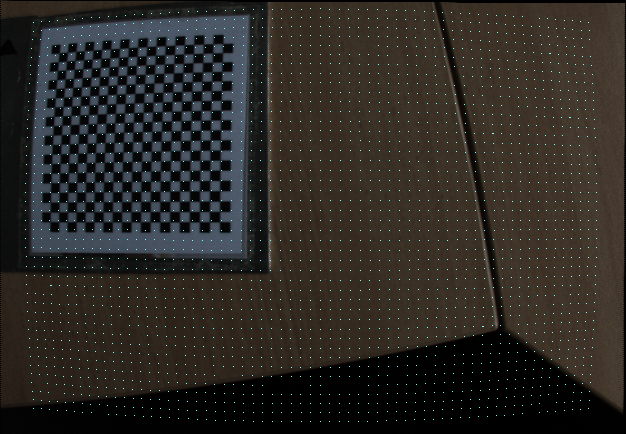
\includegraphics[width=1\textwidth]{Figs/SampPatternOrig}
	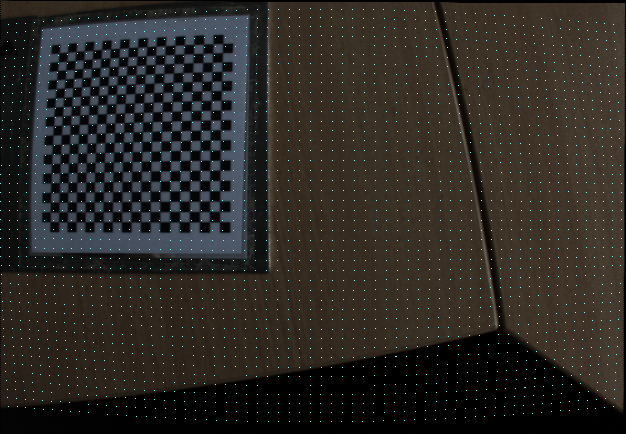
\includegraphics[width=1\textwidth]{Figs/SampPatternWide}
	\caption{The default and adjusted sampling patterns.  Here the sampling pattern has been stretched horizontally, incorporating more of the measured image, but yielding rectangular pixels. The following figure shows the result of applying each of these.}
	\label{fig_AdjustRectIntrinsic}
\end{figure}

\begin{figure}[tbhp]
	\centering
	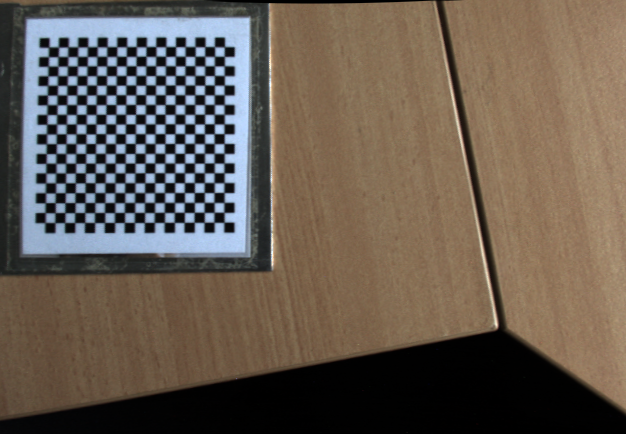
\includegraphics[width=1\textwidth]{Figs/IllumRectDefault}
	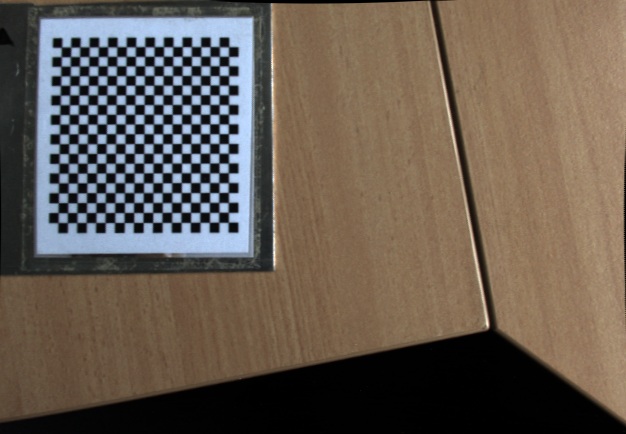
\includegraphics[width=1\textwidth]{Figs/IllumRectNonsquarePix}
	\caption{Rectification applied with the default and adjusted sampling patterns described in the previous figure.}
	\label{fig_AdjustRectIntrinsicResults}
\end{figure}


%-----------------------------
\begin{appendices}
\newpage
\section{Working with Lytro Files}
\label{sect_LytroFiles}

%----------------
\subsection{Extracting White Images}
\label{sect_LytroFiles_Cal}

Every camera has a unique database of white images needed in decoding.  On Windows machines, the white image data is found in a folder of the form
\begin{Verbatim} 
<drive_letter>:\Users\<username>\AppData\Local\Lytro\cameras\ ...
    sn-<serial_number>
\end{Verbatim}
while on a MAC, the relevant location is (on Mac OS 10.10.2 running Lytro Desktop 4.1.2)
\begin{Verbatim} 
/Users/<username>/Library/Application Support/Lytro/cameras/sn-<serial_number>
\end{Verbatim}
note that for previous versions of the MAC software these files were stored at
\begin{Verbatim} 
/Users/<username>/Lytro.lytrolib/cameras/sn-<serial_number>
\end{Verbatim}
A concrete example on a Windows machine is
\begin{Verbatim} 
C:\Users\Bob\AppData\Local\Lytro\cameras\sn-A000424242
\end{Verbatim}

The Lytro Illum can save its white images in a compressed file on its SDCard as part of the ``pairing process'' -- see the Lytro literature on creating this ``Pairing Data''.  The data folder or pairing data file contain files named \SymbolText{data.C.0}, \SymbolText{data.C.1} and so on. These are in a Lytro-specific storage format, and can be unpacked using \CiteFunc{LFUtilUnpackLytroArchive}.  

For example, after uncompressing the pairing data or copying the contents of the data folder into \SymbolText{Cameras/<YourSerial>/WhiteImages}, run \CiteFunc{LFUtilUnpackLytroArchive} from the top of the Samples folder.  The function will by default search the \SymbolText{Cameras} folder for all archives and unpack them.

Of the resulting extracted files, those we are interested in have names like
\begin{Verbatim} 
MOD_0000.RAW
MOD_0000.TXT
MOD_0001.RAW
MOD_0001.TXT
...
\end{Verbatim}

The \SymbolText{raw} files are white images corresponding to a variety of zoom and focus settings, while the \SymbolText{txt} files contain the metadata we require to sort out which is which. The other files contain a wealth of information about your Lytro, but are not utilized in this revision of the toolbox.  Once unpacked, you may safely remove the copied data.C.* files.

%----------------
\subsection{Locating Picture Files}
\label{sect_LytroFiles_Pict}

The toolbox can read Lytro LFP files directly using the function \CiteFunc{LFReadLFP}.  The toolbox is also compatible with \SymbolText{.raw} files extracted using an external LFP tool.

Lytro Desktop version 4 and higher make it easy to find LFP files, as they are stored in your operating system's default Pictures folder -- look for a folder of the form\\ \SymbolText{My Pictures/Lytro Desktop/Libraries/Lytro Library.lytrolibrary/}.  The picture library takes on a complex directory structure, with many sub-folders.  You may copy this structure directly into your working folder -- the toolbox will recursively search sub-folders when decoding light fields.  

The desktop software can also export light fields to a location of your choice.

If working with an Illum, you may copy the files straight off the camera, as it directly exposes its file system over USB.

If you're running an older versions of the Lytro Desktop software, Lytro picture files may be found in an \SymbolText{images} folder alongside the \SymbolText{cameras} folder where the white images are stored. i.e.\  on a Windows machine the default location is
\begin{Verbatim} 
<drive_letter>:\Users\<username>\AppData\Local\Lytro\images\*
\end{Verbatim}
and on a MAC it's
\begin{Verbatim} 
/Users/<username>/Lytro.lytrolib/images/*
\end{Verbatim}
where the `*' at the end takes on numerical values, like \SymbolText{01}, \SymbolText{02} and so on. 

%----------------
\subsubsection{LFP, LFR, lfp or lfr?}

The Lytro LFP is a container format, and may contain one of several types of data.  The files containing light fields are generally obvious based on their size -- about 16~MBytes for the F01, and 55~MBytes for the Illum.  The file extension varies based on the source of the files, with exported files, on-camera files and image library files variously taking on the four variants of extension shown in this section's heading.  

By default, \CiteFunc{LFUtilDecodeLytroFolder} recursively searches for files with any of these extensions, as well as the \SymbolText{raw} files employed by previous toolbox versions, and decodes anything it can make sense of.  Focal stacks and other files are also stored as \SymbolText{.lfp} files, and \CiteFunc{LFUtilDecodeLytroFolder} will ignore these files.


%----------------
\subsubsection{Thumbnails}

Thumbnails are built into some LFP files.  The function \CiteFunc{LFUtilExtractLFPThumbs} extracts thumbnails and saves them to disk.



%-----------------------------
\newpage
\section{Upgrading from 0.4}
\label{sect_Upgrading}

There have been minor performance improvements to how white images are analyzed to build grid files, and to how calibration distortion parameters get applied.

For those not using calibration or rectification, no action is required. Re-doing white image analysis will result in a small improvement in decoded light field quality.

Users employing calibration / rectification should not use previously generated calibration files with the new toolbox, and should reprocess their calibrations.

\subsection{Reprocessing White Images}
\CiteFunc{LFUtilProcessWhiteImages} fits a grid to each of the white images in the \SymbolText{Cameras} folder. To force it to redo this process, pass in a \SymbolText{FileOptions} parameter with the \SymbolText{ForceRedo} field set to true. Alternatively, delete all the \SymbolText{.grid.mat} files and the \SymbolText{WhiteImageDatabase.mat} file in the Cameras folder, then run white image analysis.

After new grid models are generated, every future image decode will benefit from the improved grid fit.

\subsection{Reprocessing Calibrations}
It is not recommended to rectify files using calibrations built using earlier toolbox versions, as interpretation of distortion parameters has changed.

First, reprocess white images as above, and re-decode calibration files, to benefit from the improved grid fit. Then, remove \SymbolText{CalibrationDatabase.mat}, and either use function parameters to force the calibration to redo previously complete steps, or delete generated files and re-run calibration. The relevant parameters to \CiteFunc{LFUtilCalLensletCam} are \SymbolText{CalOptions.ForceRedoCornerFinding} and \SymbolText{CalOptions.ForceRedoInit}. Or, if removing files, the relevant files to remove are \SymbolText{CheckerboardCorners.mat},\\ \SymbolText{CalInfo.json}, and \SymbolText{*\_\_CheckerCorners.mat}.

Once complete, run \CiteFunc{LFUtilProcessCalibrations}.


%-----------------------------
\newpage
\section{Function Reference}

This is a partial list of top-level functions organized by task. See also 
\begin{Verbatim} 
help <LFToolbox top folder name>
\end{Verbatim} 
for a more complete list. Refer to the documentation in each function for further information. The SupportFunctions folder contains additional functions used internally by the toolbox.

%------------------------------------------------------------
\NewFunctionHeading{Decoding}
%------------------------------------------------------------
\NewFunctionEntry{LFLytroDecodeImage}{}
{Decode a Lytro image from an \SymbolText{LFP} or \SymbolText{raw} file. Can be called directly to decode a single image into memory, or called indirectly through \CiteFunc{LFUtilDecodeLytroFolder}.}

\NewFunctionEntry{LFUtilDecodeLytroFolder}{}
{Utility for decoding, colour correcting and rectifying Lytro imagery. Can process multiple light fields; recursively searches folder structures; accepts filename specifications including wildcards. Selects appropriate white images and calibration files from multiple cameras across multiple zoom and focus settings. Will incrementally apply operations to files so that, for example, previously-decoded light fields can be incrementally colour-corrected, rectified or both without needing to repeat operations. Results are saved to disk. See Figs.~\ref{fig_ExampleDecodeAndColourCorrectOutput}, \ref{fig_RectificationDetail} and \ref{fig_CalibrationExampleRectification} for example output.

Demonstrates \CiteFunc{LFLytroDecodeImage}, \CiteFunc{LFColourCorrect}, \CiteFunc{LFHistEqualize}, and \CiteFunc{LFCalRectifyLF}.

Decoding relies on a white image database having been constructed by \CiteFunc{LFUtilProcessWhiteImages}, and rectification similarly relies on a calibration database having been created by \CiteFunc{LFUtilProcessCalibrations}.}

\NewFunctionEntry{LFUtilProcessWhiteImages}{}
{Processes a folder populated with white images, generating a grid model (\SymbolText{.grid.json}) for each, and a white image database (\SymbolText{WhiteFileDatabase.mat}) used to select the white image appropriate to a light field. Dark images are detected and skipped.}

%------------------------------------------------------------
\EndFunctionHeading
\NewFunctionHeading{Filtering}
%------------------------------------------------------------
\NewFunctionEntry{LFBuild2DFreqFan}{}
{Construct a 2D fan filter in the frequency domain.  Apply this filter with \CiteFunc{LFFilt2DFFT}.}
\NewFunctionEntry{LFBuild2DFreqLine}{}
{Construct a 2D line filter in the frequency domain.  The cascade of two line filters, applied in s,u and in t,v, is identical to a 4D planar filter, e.g.\ that constructed by \CiteFunc{LFBuild4DFreqPlane}.   Apply this filter with \CiteFunc{LFFilt2DFFT}.}
\NewFunctionEntry{LFBuild4DFreqDualFan}{}
{Construct a 4D dual-fan filter in the frequency domain.    Apply this filter with \CiteFunc{LFFilt4DFFT}.}
\NewFunctionEntry{LFBuild4DFreqHypercone}{}
{Construct a 4D hypercone filter in the frequency domain.   Apply this filter with \CiteFunc{LFFilt4DFFT}.}
\NewFunctionEntry{LFBuild4DFreqHyperfan}{}
{Construct a 4D hyperfan filter in the frequency domain. This is useful for selecting objects over a range of depths from a lightfield, i.e.\ volumetric focus.  Apply this filter with \CiteFunc{LFFilt4DFFT}.}
\NewFunctionEntry{LFBuild4DFreqPlane}{}
{Construct a 4D plane filter in the frequency domain.  This is useful for selecting objects at a single depth from a lightfield, and is similar in effect to refocus using, for example, the shift sum filter \CiteFunc{LFFiltShiftSum}.  Apply this filter with \CiteFunc{LFFilt4DFFT}.}

\NewFunctionEntry{LFDemoBasicFiltLytroF01}{}
{Demonstrates some of the basic filters on Lytro F01-captured imagery.}
\NewFunctionEntry{LFDemoBasicFiltIllum}{}
{Demonstrates some of the basic filters on Lytro Illum-captured imagery.}
\NewFunctionEntry{LFDemoBasicFiltGantry}{}
{Demonstrates some of the basic filters on Stanford light field archive light fields.}
\NewFunctionEntry{LFDemoRefocusSuperres}{\NewTag}
{Demonstrates linear refocus-based super-resolution, see Sect.~\ref{sect_SuperResTour}.}


\NewFunctionEntry{LFFilt2DFFT}{}
{Applies a 2D frequency-domain filter to a 4D light field using the FFT.}
\NewFunctionEntry{LFFilt4DFFT}{}
{Applies a 4D frequency-domain filter using the FFT.}
\NewFunctionEntry{LFFiltShiftSum}{}
{The shift sum filter is a spatial-domain depth-selective filter, with an effect similar to planar focus. \NewText: Use the UpsampRate parameter for linear refocus super-resolution.}


%------------------------------------------------------------
\EndFunctionHeading
\NewFunctionHeading{Image Adjustment}
%------------------------------------------------------------

\NewFunctionEntry{LFColourCorrect}{}
{Applies a colour balance vector, an RGB colour correction matrix, and gamma correction. Usage is demonstrated in \CiteFunc{LFUtilDecodeLytroFolder}.}

\NewFunctionEntry{LFHistEqualize}{}
{Adjusts the brightness of a light field based on histogram stretching. Capable of handling colour and monochrome images -- colour images are converted to HSV, and the value channel is equalized. Capable of handling different input dimensionalities including 2D images and 4D light fields. If a weight channel is present as a fourth colour channel, it is used to ignore zero-weight pixels. Usage is demonstrated in \CiteFunc{LFUtilDecodeLytroFolder}.}

%------------------------------------------------------------
\EndFunctionHeading
\NewFunctionHeading{Visualization}
%------------------------------------------------------------
\NewFunctionEntry{LFDisp}{}
{Convenience function to display a static, 2D slice of a light field.  The centermost image is taken in $s$ and $t$.  Also works with 3D arrays of images and 2D images. Can be nested as demonstrated in Sect.~\ref{sect_DisplayingTour}.}

\NewFunctionEntry{LFDispLawnmower}{\NewTag}
{Similar to \CiteFunc{LFDispVidCirc}, but visits every light field view in sequence following horizontal and vertical lawnmower patterns.}

\NewFunctionEntry{LFDispMousePan}{}
{Interactively display 2D slices of the light field with a parallax effect. Click and drag in the image to change the point of view. An optional parameter controls the display size. Note that darkening at the edges of lenslet-based light fields mean that the effect is best near the center of the spatial range.}

\NewFunctionEntry{LFDispProj}{\NewTag}
{Displays the light field by projecting it onto a plane.}

\NewFunctionEntry{LFDispProjSubfigs}{\NewTag}
{Uses \CiteFunc{LFDispProj} to display six different projections of the light field.}

\NewFunctionEntry{LFDispTiles}{\NewTag}
{Displays the light field as a 2D tiling of 2D images.}

\NewFunctionEntry{LFDispTilesSubfigs}{\NewTag}
{Uses \CiteFunc{LFDispTiles} to display six different tilings of the light field.}

\NewFunctionEntry{LFDispVidCirc}{}
{Animated display showing 2D slices of the light field, similar to \CiteFunc{LFDispMousePan} except the motion is preset to a circular path. Optional parameters include the radius of the circular path, animation speed, and display size.}

\NewFunctionEntry{LFFigure}{}
{Replacement for Matlab's ``figure'' which doesn't steal focus, originally sfigure by Daniel Eaton.}

%------------------------------------------------------------
\EndFunctionHeading
\NewFunctionHeading{Calibration}
%------------------------------------------------------------
\NewFunctionEntry{LFCalDispEstPoses}{}
{Visualize camera pose estimates. Called by \CiteFunc{LFUtilCalLensletCam}.}

\NewFunctionEntry{LFCalDispRectIntrinsics}{}
{Helper for setting up and visualizing intrinsics requested in rectification, see also \CiteFunc{LFRecenterIntrinsics}.}

\NewFunctionEntry{LFCalRectifyLF}{}
{Applies a calibration to rectify a light field. The desired intrinsic matrix can be provided, or computed automatically from the calibrated intrinsics. Demonstrated by \CiteFunc{LFUtilDecodeLytroFolder}.}

\NewFunctionEntry{LFRecenterIntrinsics}{}
{Recenters a light field intrinsic matrix, useful for modifying intrinsics requested in \CiteFunc{LFCalRectifyLF}, see \CiteFunc{LFCalDispRectIntrinsics}.}

\NewFunctionEntry{LFUtilCalLensletCam}{}
{Runs through all the steps of a lenslet-based camera calibration.}

\NewFunctionEntry{LFUtilProcessCalibrations}{}
{Builds a database of calibrations to allow selection of the appropriate calibration for a given light field.}

%------------------------------------------------------------
\EndFunctionHeading
\NewFunctionHeading{File I/O}
%------------------------------------------------------------

\NewFunctionEntry{LFFindFilesRecursive}{}
{Recursively searches a folder for files matching one or more patterns.  Refer to this to understand the path parameters to \CiteFunc{LFUtilDecodeLytroFolder}, \CiteFunc{LFUtilExtractLFPThumbs} and  \CiteFunc{LFUtilUnpackLytroArchive}.}

\NewFunctionEntry{LFReadESLF}{\NewTag}
{Reads ESLF light field images, as generated by the Lytro Power Tools.}

\NewFunctionEntry{LFReadGantryArray}{}
{Loads gantry-style light fields, e.g.\ the Stanford gantry light fields found at \url{http://lightfield.stanford.edu}.}

\NewFunctionEntry{LFReadLFP}{}
{Reads Lytro \SymbolText{lfp}/\SymbolText{lfr} light field files.}

\NewFunctionEntry{LFReadMetadata}{}
{Reads \SymbolText{json} files.}

\NewFunctionEntry{LFReadRaw}{}
{Reads 10, 12 and 16-bit \SymbolText{raw} image files.}

\NewFunctionEntry{LFWriteESLF}{\NewTag}
{Writes ESLF light field images.}

\NewFunctionEntry{LFWriteMetadata}{}
{Writes \SymbolText{json} files.}

%------------------------------------------------------------
\EndFunctionHeading
\NewFunctionHeading{Utility / Convenience}
%------------------------------------------------------------
\NewFunctionEntry{LFConvertToInt}{\NewTag}
{Converts to \SymbolText{uint8} or \SymbolText{uint16}, with automatic scaling.}

\NewFunctionEntry{LFConvertToFloat}{}
{Converts to \SymbolText{single} or \SymbolText{double}, with automatic scaling.}

\NewFunctionEntry{LFMatlabPathSetup}{}
{Sets up the Matlab path to include the LF Toolbox. This must be re-run every time Matlab restarts, so consider adding a line to \SymbolText{startup.m} as shown in Sect.~\ref{sect_Installation}.
}

\NewFunctionEntry{LFUtilUnpackLytroArchive}{}
{Extracts white images and other files from a multi-volume Lytro archive.}

\NewFunctionEntry{LFUtilExtractLFPThumbs}{}
{Extracts thumbnails from LFP files and writes them to disk.}

\EndFunctionHeading
%------------------------------------------------------------




\end{appendices}
\end{document}
